\chapter{Compiler}
\label{ch:compiler}
\section{Introduction}
\label{sec:cintro}
The compiler is the primary tool of the system builder. It therefore plays a prominent role in the
Oberon System, although it is not part of the basic system. Instead, it constitutes a tool module - an
application - with a single command: Compile. It translates program texts into machine code.
Therefore, it is as a program inherently machine-dependent; it acts as the interface between source
language and target computer.

In order to understand the process of compilation, the reader needs to be familiar with the source
language Oberon defined in Appendix 1, and with the target computer RISC, defined in Appendix 2.

The language is defined as an infinite set of sequences of symbols taken from the language's
vocabulary. It is described by a set of equations called syntax. Each equation defines a syntactic
construct, or more precisely, the set of sequences of symbols belonging to that construct. It
specifies how that construct is composed of other syntactic constructs. The meaning of programs is
defined in terms of semantic rules governing each such construct.

Compilation of a program text proceeds by analyzing the text and thereby decomposing it
recursively into its constructs according to the syntax. When a construct is identified, code is
generated according to the semantic rule associated with the construct. The components of the
identified construct supply parameters for the generated code.

It follows that we distinguish between 2 kinds of actions: analyzing steps and code generating
steps. In a rough approximation we may say that the former are source language dependent and
target computer independent, whereas the latter are source language independent and target
computer dependent. Although reality is somewhat more complex, the module structure of this
compiler clearly reflects this division. The main module of the compiler is ORP (for Oberon to RISC
Parser) It is primarily dedicated to syntactic analysis, parsing. Upon recognition of a syntactic
construct, an appropriate procedure is called the code generator module ORG (for Oberon to RISC
Generator). Apart from parsing, ORP checks for type consistency of operands, and it computes the
attributes of objects identified in declarations.

Whereas ORP mirrors the source language and is independent of a target computer, ORG reflects
the target computer, but is independent of the source language.

Oberon program texts are regarded as sequences of symbols rather than sequences of characters.
Symbols themselves, however, are sequences of characters. We refrain from explaining the
reasons for this distinction, but mention that apart from special characters and pairs such as +, \&,
<=, also identifiers, numbers, and strings are classified as symbols. Furthermore, certain capital
letter sequences are symbols, such as IF, END, etc. Each time the syntax analyzer (parser)
proceeds to read the next symbol, it does this by calling procedure \verb|Get|, which constitutes
the so-called scanner residing in module ORS (for Oberon to RISC Scanner). It reads from the source
text as many characters as needed to recognize the next symbol.

In passing we note that the scanner alone reflects the definition of symbols in terms of characters,
whereas the parser is based on the notion of symbols only. The scanner implements the abstraction
of symbols. The recognition of symbols within a character sequence is called \emph{lexical analysis}.

Ideally the recognition of any syntactic construct, say \verb|A|, consisting of subconstructs, say
\verb|B1|, \verb|B2|, ..., \verb|Bn|, leads to the generation of code that depends only on
\begin{enumerate}
  \item the semantic rules associated with \verb|A|, and
  \item on (attributes of) \verb|B1|, \verb|B2|, ..., \verb|Bn|.
\end{enumerate}
If this condition is satisfied, the construct is said to be \emph{context-free}, and if all constructs
of a language are context-free, then also the language is context-free. Syntax and semantics of Oberon
adhere to this rule, although with a significant exception. This exception is embodied by the notion
of declarations. The declaration of an identifier, say \verb|x|, attaches permanent properties to
\verb|x|, such as the fact that \verb|x| denotes a variable and that its type is \verb|T|. These
properties are "invisible" when parsing a statement containing \verb|x|, because the declaration of
\verb|x| is not also part of the statement. The "meaning" of identifiers is thus inherently
\emph{context-dependent}.

Context-dependence due to declarations is the immediate reason for the use of a global data
structure which represents the declared identifiers and their properties (attributes). Since this
concept stems from early assemblers where identifiers (then called symbols) were registered in a
linear table, the term symbol table tends to persist for this structure, although in this compiler
it is considerably more complex than an array. Basically, it grows during the processing of
declarations, and it is searched while expressions and statements are processed. Procedures for
building and for searching are contained in module ORB.

A complication arises from the notion of exports and imports in Oberon. Its consequence is that the
declaration of an identifier \verb|x| may be in a module, say \verb|M|, different from where \verb|x|
is referenced. If \verb|x| is exported, the compiler includes \verb|x| together with its attributes
in the symbol file of the compiled module \verb|M|. When compiling another module which imports
\verb|M|, that symbol file is read and its data are incorporated into the symbol table. Procedures
for reading and writing symbol files are contained in module ORB, and no other module relies on
information about the structure of symbol files.

The syntax is precisely and rigorously defined by a small set of syntactic equations. As a result,
the parser is a reasonably perspicuous and short program. In spite of the high degree of regularity
of the target computer, the process of code generation is more complicated, as shown by module ORG.

The resulting module structure of the compiler is shown in Fig. \ref{fig:modstruct} in a slightly
simplified manner.  In reality OCS is imported by all other modules due to their need for procedure
\verb|OCS.Mark|. This, however, will be explained later.
\begin{figure}[h!]
  \centering
  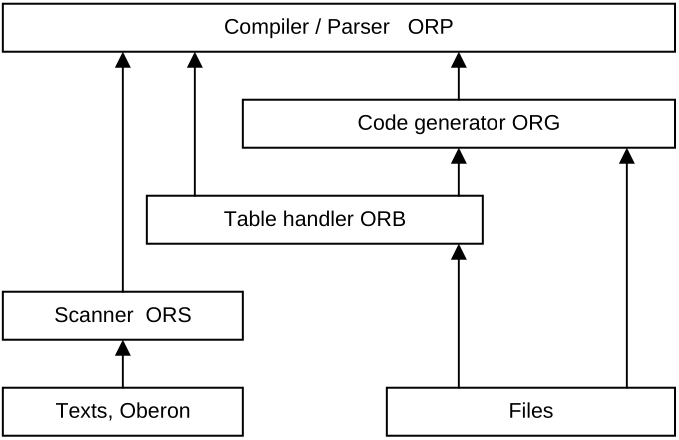
\includegraphics[width=.75\textwidth]{i/C/1.png}
  \caption{Compiler's module structure}
  \label{fig:modstruct}
\end{figure}

\section{Code patterns}
\label{sec:codeptn}
Before it is possible to understand how code is generated, one needs to know which code is
generated. In other words, we need to know the goal before we find the way leading to the goal. A
fairly concise description of this goal is possible due to the structure of the language. As explained
before, semantics are attached to each individual syntactic construct, independent of its context.
Therefore, it suffices to list the expected code - instead of an abstract semantic rule - for each
syntactic construct.

As a prerequisite to understanding the resulting instructions and in particular their parameters, we
need to know where declared variables are stored, i.e. which are their addresses. This compiler
uses the straight-forward scheme of sequential allocation of consecutively declared variables. An
address is a pair consisting of a base address (in a register) and an offset. Global variables are
allocated in the module's data section and the respective base address register is SB (Static Base,
see Chapter 6). Local variables are allocated in a procedure activation record on the stack; the
respective base register is SP (Stack Pointer). Offsets are positive integers.

The amount of storage needed for a variable (called its \emph{size}) is determined by the variable's
type.  The sizes of basic types are prescribed by the target computer's data representation.
The following holds for the RISC processor:
\begin{table}[h!]
  \centering
  \begin{tabular}{c c}
    Types                         & Size \\
    BYTE, CHAR, BOOL              & 1 \\
    INT, REAL, SET, POINTER, PROC & 4
  \end{tabular}
\end{table}

The size of an array is its element's multiplied by the number of elements; The size of a record is
the sum of all its fields'.

A complication arises due to so-called alignment. By alignment is meant the adjustment of an
address to a multiple of the variable's size. Alignment is performed for variable addresses as well
as for record field offsets. The motivation for alignment is the avoidance of double memory
references for variables being "distributed" over 2 adjacent words. Proper alignment enhances
processing speed quite significantly. Variable allocation using alignment is shown by the example
in Fig. \ref{fig:varalign}.
\begin{figure}[h!]
  \centering
  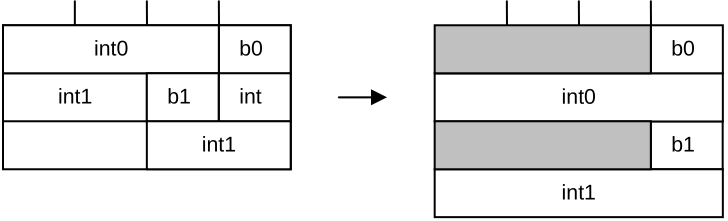
\includegraphics[width=.75\textwidth]{i/C/2.png}
  \caption{Alignment of variables}
  \label{fig:varalign}
\end{figure}

We note in passing that a reordering of the four variables lessens the number of unused bytes, as
shown in Fig. \ref{fig:varorder}.
\begin{figure}[h!]
  \centering
  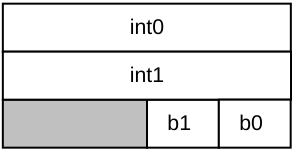
\includegraphics[width=.25\textwidth]{i/C/3.png}
  \caption{Improved order of variables}
  \label{fig:varorder}
\end{figure}

Memory instructions compute the address as the sum of a register (base) and an offset constant.
Local variables use the stack pointer SP (R14) as base, global variables the static base SB (R13)
Every module has its own SB value, and therefore access to global (and imported) variables
requires 2 instructions, one for fetching the base value, and one for loading or storing data. If the
compiler can determine, whether the correct base value has already been loaded into the SB
register, the former instruction is omitted.

The first 7 sample patterns contain global variables only, and their base SB is assumed to hold the
appropriate value. Parameters of branch instructions denote jump distances from the instruction's
own location (PC-relative).

\subsection{Assignment of constants}
\label{ssc:ptn1}
We begin with a simple example of assigning constants to variables. The variables used in this example
are global; their base register is \verb|SB|. Each assignment results in a single instruction.
The constant is embedded within the instruction as a literal operand.
\begin{verbatim}
  MODULE Pattern1;
    VAR ch: CHAR;     0
         k: INT ;     4
         x: REAL;     8
         s: SET ;    12
  BEGIN                         module entry code    
    ch := "0";       40000030   MOV  R0 R0 30H
                     B0D00000   STR  R0 SB 0
     k := 10 ;       4000000A   MOV  R0 R0 10
                     A0D00004   STR  R0 SB 4
     x := 1.0;       60003F80   MOV' R0 R0 3F800000H
                     A0D00008   STR  R0 SB 8
     s := {0, 4, 8}  40000111   MOV  R0 R0 111H
                     A0D0000C   STR  R0 SB 12
  END Pattern1.                 module exit code
\end{verbatim}

\subsection{Simple expressions}
The result of an expression containing operators is always stored in a register before it is assigned
to a variable or used in another operation.

Registers for intermediate results are allocated sequentially in ascending order \verb|R0|, \verb|R1|,
..., \verb|R11|.  Integer multiplication and division by powers of 2 are represented by shifts (LSL,
ASR). Similarly, the modulus by a power of 2 is obtained by masking off leading bits. The operations
of set union, difference, and intersection are represented by logical operations (OR, AND).
\begin{verbatim}
  MODULE Pattern2;
    VAR i, j, k, n: INT ;   0,  4,  8, 12
              x, y: REAL;          16, 20
           s, t, u: SET ;      24, 28, 32
  
  BEGIN i := (i + 1) * (i - 1);   LDR  R0 SB 0
                                  ADD  R0 R0 1
                                  LDR  R1 SB 0
                                  SUB  R1 R1 1
                                  MUL  R0 R0 R1
                                  STR  R0 SB 0
        k := k DIV 17         ;   LDR  R0 SB 8
                                  DIV  R0 R0 17
                                  STR  R0 SB 8
        k := 8 * n            ;   LDR  R0 SB 12
                                  LSL  R0 R0 3
                                  STR  R0 SB 8
        k := n DIV 2          ;   LDR  R0 SB 12
                                  ASR  R0 R0 1
                                  STR  R0 SB 8
        k := n MOD 16         ;   LDR  R0 SB 12
                                  AND  R0 R0 15
                                  STR  R0 SB 8
        x := -y / (x - 1.0)   ;   LDR  R0 SB 16
                                  MOV' R1 R0 3F80H
                                  FSB  R0 R0 R1
                                  LDR  R1 SB 20
                                  FDV  R0 R1 R0
                                  MOV  R1 R0 0
                                  FSB  R0 R1 R0
                                  STR  R0 SB 16
        s := s + t * u            LDR  R0 SB 28
                                  LDR  R1 SB 32
                                  AND  R0 R0 R1 
                                  LDR  R1 SB 24
                                   OR  R0 R1 R0
                                  STR  R0 SB 24
  END Pattern2.
\end{verbatim}

\subsection{Indexed variables}
References to elements of arrays make use of the possibility to add an index value to an offset.
The index must be present in a register and be multiplied by the size of the array elements. (For
integers with size 4 this is done by a shift of 2 bits). Then this index is checked whether it lies
within the bounds specified in the array's declaration. This is achieved by a comparison, actually
a subtraction, and a subsequent branch instruction causing a trap, if the index is either negative
or beyond the upper bound.

If the reference is to an element of a multi-dimensional array (matrix), its address computation
involves several multiplications and additions. The address of an element $A[i_{k-1}, ..., i_1, i_0]$
of a $k$-dimensional array $A$ with lengths $n_{k-1}, ..., n_1, n_0$ is

\[ \text{adr}(A) + (( ... ((i_{k-1} * n_{k-2}) + i_{k-2}) * n_{k-3} + ... ) * n_1 + i_1) * n_0 + i_0 \]

Note that for index checks CMP is written instead of SUB to mark that the subtraction is merely a
comparison, that the result remains unused and only the condition flag registers hold the result.
\begin{verbatim}
  MODULE Pattern3;
    VAR i, j, k, n:         INT;   0, 4, 8, 12 
     a: ARRAY 10         OF INT;            16
     x: ARRAY 10, 10     OF INT;            56
     y: ARRAY 10, 10, 10 OF INT;           456

  BEGIN      k := a[i];     LDR R0 SB 0
                            CMP R1 R0 10
                            BLHI R12
                            LSL R0 R0 2
                            ADD R0 SB R0
                            LDR R0 R0 16
                            STR R0 SB 8
             n := a[5];     LDR R0 SB 36
                            STR R0 SB 12
    x[i,    j] :=   2 ;     LDR R0 SB 0
                            CMP R1 R0 10
                            BLHI R12
                            MUL R0 R0 40
                            ADD R0 SB R0
                            LDR R1 SB 4
                            CMP R2 R1 10
                            BLHI R12
                            LSL R1 R1 2
                            ADD R0 R0 R1
                            MOV R1 R0 2
                            STR R1 R0 56
    y[i, j, k] :=   3 ;     LDR R0 SB 0
                            CMP R1 R0 10
                            BLHI R12
                            MUL R0 R0 400
                            ADD R0 SB R0
                            LDR R1 SB 4
                            CMP R2 R1 10
                            BLHI R12
                            MUL R1 R1 40
                            ADD R0 R0 R1
                            LDR R1 SB 8
                            CMP R2 R1 10
                            BLHI R12
                            LSL R1 R1 2
                            ADD R0 R0 R1
                            MOV R1 R0 3
                            STR R1 R0 456  
    y[3, 4, 5] :=   6       MOV R0 R0 6
                            STR R0 SB 1836
  END Pattern3.
\end{verbatim}

\subsection{RECORD fields and pointers}
\label{ssc:ptn4}
Fields of records are accessed by computing the sum of the record's (base) address and the field's
offset. If the record variable is statically declared, the sum is computed by the compiler.
\begin{verbatim}
  MODULE Pattern4;
    TYPE Ptr = POINTER TO Node;
        Node = RECORD num: INT;      0      
          name: ARRAY 8 OF CHAR;     4
          next: Ptr                 12
        END ;                       
    VAR p, q: Ptr ;             12, 16
           r: Node;                 20
  BEGIN
    r.num       := 10 ;   MOV R0 R0 10               
                          STR R0 SB 20
    p.num       :=  6 ;   LDR R0 SB 12 (p)
                          MOV R1 R0  6
                          STR R1 R0  0
    p.name[7]   := "0";   LDR R0 SB 12
                          MOV R1 R0 30H
                          STR R1 R0 11 (4+7)
    p.next      :=  q ;   LDR R0 SB 12
                          LDR R1 SB 16
                          STR R1 R0 12
    p.next.next := NIL    LDR R0 SB 12 (p)
                          LDR R0 R0 12 (p.next)
                          MOV R1 R0  0 (NIL)
                          STR R1 R0 12 (p.next.next)
  END Pattern4.
\end{verbatim}

\subsection{Boolean expressions, IF statements}
\label{ssc:ptn5}
Conditional statements imply that parts of them are skipped. This is done by the use of branch
instructions whose operand specifies the distance of the branch. The instructions refer to the
condition-register as an implicit operand. Its value is determined by a preceding instruction,
typically a compare or a bit-test instruction.

The Boolean operators \verb|&| and \verb|OR| are purposely not defined as total functions, but
rather by the equations
\begin{verbatim}
  p  & q = if p then q else FALSE
  p OR q = if p then TRUE else q
\end{verbatim}

Consequently, Boolean operators must be translated into branches too. Evidently, branches
stemming from if statements and branches stemming from Boolean operators should be merged, if
possible. The resulting code therefore does not necessarily mirror the structure of the if statement
directly, as can be seen from the code in Pattern5. We must conclude that code generation for
Boolean expressions differs in some aspects from that for arithmetic expressions.

The example of Pattern5 is also used to exhibit the code resulting from the standard procedures
INC, DEC, INCL, and EXCL. These procedures provide an opportunity to use shorter code in those
cases where a single 2-operand instruction suffices, i.e. when one of the arguments is identical
with the destination.

\begin{verbatim}
  MODULE Pattern5;
    VAR n: INT; s: SET;           0, 4
  BEGIN
    IF n = 0 THEN                  LDR R0 SB 0     
                                   CMP R0 R0 0
                                   BNE 3
      INC(n)                       LDR R0 SB 0
                                   ADD R0 R0 1
                                   STR R0 SB 0
    END ;                          
    IF (n >= 0) & (n < 100) THEN   LDR SB R0 ...
                                   LDR R0 SB 0 (n)
                                   CMP R0 R0 0
                                   BLT 6
                                   LDR R0 SB 0
                                   CMP R0 R0 100
                                   BGE 3
      DEC(n)                       LDR R0 SB 0
                                   SUB R0 R0 1
                                   STR R0 R0 0
    END ;                          
    IF ODD(n) OR (n IN s) THEN     LDR SB R0 ...
                                   LDR R0 SB 0 (n)
                                   AND R0 R0 1
                                   BNE 5
                                   LDR R0 SB 4 (s)
                                   LDR R1 SB 0
                                   ADD R1 R1 1
                                   ROR R0 R0 R1
                                   BPL 2
      n := -1000                   MOV R0 R0 -1000
                                   STR R0 SB 0
    END ;                          
    IF n < 0 THEN                  LDR SB R0 ...
                                   LDR R0 SB 0
                                   CMP R0 R0 0
                                   BGE 3
      s := {}                      MOV R0 R0 0 {}
                                   STR R0 SB 4
                                   B 17
    ELSIF n < 10 THEN              LDR SB R0 ...
                                   LDR R0 SB 0
                                   CMP R0 R0 10
                                   BGE 3
      s := {0}                     MOV R0 R0 1
                                   STR
                                   B 10
    ELSIF n < 100 THEN             LDR SB R0 ...
                                   LDR R0 SB 0
                                   CMP R0 R0 100
                                   BGE 3
      s := {1}                     MOV R0 R0 2
                                   STR R0 SB 4
                                   B 3
    ELSE                           
      s := {2}                     MOV R0 R0 4
                                   LDR SB R0 ...
                                   STR R0 SB 4
    END
  END Pattern5.
\end{verbatim}

\subsection{WHILE and REPEAT statements}
\begin{verbatim}
  MODULE Pattern6;
    VAR i: INT;
  BEGIN i := 0;            MOV R0 R0 0   
                           STR R0 SB 0
    WHILE i < 10 DO        LDR SB R0 ...
                           LDR R0 SB 0
                           CMP R0 R0 10
                           BGE  4
      i := i + 2           LDR R0 SB 0
                           ADD R0 R0 2
                           STR R0 SB 0
    END ;                  B   -8
    REPEAT i := i - 1      LDR SB R0 ...
                           LDR R0 SB 0
                           SUB R0 R0 1
                           STR R0 SB 0
    UNTIL i = 0            LDR R0 SB 0
                           CMP R0 R0 0
                           BNE -7
  END Pattern6.
\end{verbatim}

\subsection{FOR statements}
\label{ssc:ptn7}
\begin{verbatim}
  MODULE Pattern7;
    VAR i, m, n: INT;
  BEGIN
    FOR i := 0 TO n-1 DO   MOV R0 R0 0   
                           LDR R1 SB 8
                           SUB R1 R1 1
                           CMP LNK R0 R1
                           BGT  7
                           STR R0 SB 0
      m := 2*m             LDR R0 SB 4
                           LSL R0 R0 1
                           STR R0 SB 4
    END                    LDR R0 SB 0
                           ADD R0 R0 1
                           B  -11
  END Pattern7.
\end{verbatim}

\subsection{Proper procedures}
Procedure bodies are surrounded by a prolog (entry code) and an epilog (exit code). They reposition
the stack pointer SP (see Chapter 6), which holds the address of the procedure activation record on
the stack. The immediate value of the first instruction indicates the space taken by variables local
to the procedure, rounded up to the next multiple of 4.

Procedure calls use a branch and link (BL) instruction. Parameters are loaded into registers prior to
the call and pushed on the stack after the call. Every parameter occupies a multiple of 4 bytes. In
the case of value parameters the value is loaded, and in the case of VAR-parameters, the variable's
address is loaded.
\begin{verbatim}
  MODULE Pattern8;
    VAR i: INT;
    PROC P(x: INT; VAR y: INT);
      VAR z: INT;
    BEGIN          SUB SP  SP 16   adjust SP
                   STR LNK SP  0   push ret adr
                   STR R0  SP  4   push x
                   STR R1  SP  8   push @y
      z := x;      LDR R0  SP  4   x
                   STR R0  SP 12   z
      y := z       LDR R0  SP 12   z
                   LDR R1  SP  8   @y
                   STR R0  R1  0   y
    END P;         LDR LNK SP  0   pop ret adr
                   ADD SP  SP 16
                   B   R15

  BEGIN P(5, i)    MOV R0  R0  5
                   ADD R1  SB  0   @i
                   BL -14          call
  END Pattern8.
\end{verbatim}

\subsection{Functions}
They are handled in exactly the same manner as proper procedures, except that a result is returned
in register R0. If the function is called in an expression at a place where intermediate results
are held in registers, these values are put onto the stack before the call, and they are restored
after return (not shown here).
\begin{verbatim}
  MODULE Pattern9;
    VAR x: REAL;
    PROC F(x: REAL): REAL;
    BEGIN                 SUB  SP SP 8                   
                          STR LNK SP 0    push ret adr 
                          STR  R0 SP 4    push x
      IF x >= 1.0 THEN    LDR  R0 SP 4
                          MOV' R1 R0 3F80H
                          FSB  R0 R0 R1
                          BLT  4
        x := F(F(x))      LDR  R0 SP 4
                          BL  -9
                          BL  -10
                          STR  R0 SP 4
      END ;
      RETURN x            LDR  R0 SP 4
    END F;                LDR LNK SP 0     pop ret adr
                          ADD  SP SP 8
                          B   R15
  END Pattern9.
\end{verbatim}

\subsection{Dynamic ARRAYs}
Dynamic array parameters are passed by loading a descriptor on the stack, regardless of whether they
are value- or VAR- parameters. The descriptor consists of the actual variable's address and the array's
length. (Only 1-dimensional dynamic arrays are handled).

Elements of dynamic arrays are accessed like those of static arrays. However, even when the index is a
constant, the check cannot be performed by the compiler.
\begin{verbatim}
  MODULE Pattern10;
    VAR a: ARRAY 12 OF INT;
    PROC P(x: ARRAY OF INT);
      VAR i, n: INT;
    BEGIN             SUB SP SP 20              
                      STR LNK SP 0
                      STR R0 SP 4         x
                      STR R1 SP 8 x.len
      n := x[i];      LDR R0 SP 12        i
                      LDR R1 SP 8         x.len
                      CMP R2 R0 R1
                      BLHI R12
                      LSL R0 R0 2
                      LDR R1 SP 4         x
                      ADD R0 R1 R0
                      LDR R0 R0 0
                      STR R0 SP 16
      x[i+1] := n+5   LDR R0 SP 12        i
                      ADD R0 R0 1
                      LDR R1 SP 8         x.len
                      CMP R2 R0 R1
                      BLHI R12
                      LSL R0 R0 2
                      LDR R1 SP 4         x
                      ADD R0 R1 R0
                      LDR R1 SP 16        n
                      ADD R1 R1 5
                      STR R1 R0 0
    END P;            LDR LNK SP 0
                      ADD SP SP 20
                      B R15
                      
  BEGIN P(a);         ADD R0 SB 0         a
                      MOV R1 R0 12        a.len
                      BL -29
  END Pattern10.
\end{verbatim}

\subsection{SETs}
This code pattern exhibits the construction of sets. If the specified elements are constants, the set
value is computed by the compiler. Otherwise, sequences of move and shift instructions are used. Since
shift instructions do not check whether the shift count is within sensible bounds, the results are
unpredictable, if elements outside the range 0 .. 31 are involved.
\begin{verbatim}
  MODULE Pattern11;
    VAR s: SET; m, n: INT;
  BEGIN
    s := {m};                     LDR R0 SB 4     m 
                                  MOV R1 R0 1
                                  LSL R0 R1 R0
                                  STR R0 SB 0     s
    s := {0 .. n};                LDR R0 SB 8     n
                                  MOV R1 R0 -2
                                  LSL R0 R1 R0
                                  XOR R0 R0 -1
                                  STR R0 SB 0
    s := {m .. 31};               LDR R0 SB 4     m
                                  MOV R1 R0 31
                                  MOV R2 R0 -2
                                  LSL R1 R2 R1
                                  MOV R2 R0 -1
                                  LSL R0 R2 R0
                                  XOR R0 R0 R1
                                  STR R0 SB 0     s
    s := {m .. n};                LDR R0 SB 4     m
                                  LDR R1 SB 8     n
                                  MOV R2 R0 -2
                                  LSL R1 R2 R1
                                  MOV R2 R0 -1
                                  LSL R0 R2 R0
                                  XOR R0 R0 R1
                                  STR R0 SB 0     s
    IF n IN {2,3,5,7,11,13} THEN  MOV R0 R0 28ACH
                                  LDR R1 SB 8
                                  ADD R1 R1 1
                                  ASR' R0 R0 R1
                                  BPL 2
      m := 1                      MOV R0 R0 1
                                  STR R0 SB 4     m
    END
  END Pattern11.
\end{verbatim}

\subsection{Imported variables and procedures}
\label{ssc:ptn12}
When a procedure is imported from another module, its address is unavailable to the compiler. Instead,
the procedure is identified by a number obtained from the imported module's symbol file. In place of
the offset, the branch instruction holds
\begin{enumerate}
  \item the number of the imported module,
  \item the number of the imported procedure, and
  \item a link in the list of BL instructions calling an external procedure.
\end{enumerate}
This list is traversed by the linking loader, that computes the actual offset (fixup, see Chapter 6).

Imported variables are also referenced by a variable's number. In general, an access required 2
instructions. The first loads the static base register SB from a global table with the address of that
module's data section. The module number of the imported variable serves as index. The second
instruction loads the address of the variable, using the actual offset fixed up by the loader.

In the following example, modules \verb|P12a| and \verb|P12b| both export a procedure and a variable.
They are referenced from the importing module \verb|Pattern12|.
\begin{verbatim}
  MODULE P12a;
    VAR k*: INT;
  
    PROC P*;
    BEGIN k := 1
    END P;
  END P12a.
  
  MODULE P12b;
    VAR x*: REAL;
  
    PROC Q*;
    BEGIN x := 1
    END Q;
  END P12b.
  
  MODULE Pattern12;
    IMPORT P12a, P12b;
    VAR i: INT; y: REAL;
  BEGIN
    i := P12a.k;   8D10xxxx   LDR SB 1 link   P12a
                   80D00000   LDR R0 SB 0     P12a.k
                   8D00xxxx   LDR SB 0 link   Pattern12
                   A0D00000   STR R0 SB 0     Pattern12.i
    y := P12b.x;   8D20xxxx   LDR SB 2 link   P12b
                   80D00000   LDR R0 SB 0     P12b.x
                   8D00xxxx   LDR SB 0 link   Pattern12
                   A0D00004   STR R0 SB 4     Pattern12.y
  END Pattern12.
\end{verbatim}

\subsection{RECORD extensions with pointers}
Fields of a record type \verb|R1|, which is declared as an extension of a type \verb|R0|, are simply
appended to the fields of \verb|R0|, i.e. their offsets are greater than those of the fields of
\verb|R0|. When a record is statically declared, its type is known by the compiler. If the record is
referenced via a pointer, however, this is not the case. A pointer bound to a base type \verb|R0| may
well refer to a record of an extension \verb|R1| of \verb|R0|. Type tests (and type guards) allow to
test for the actual type. This requires that a type can be identified at the time of program execution.
Because the language defines name equivalence instead of structural equivalence of types, a type may
be identified by a number. We use the address of a unique type descriptor for this purpose.

Therefore, type tests consist of a simple address comparison which is very fast. Type descriptors
are stored in the module's area for data. Their address is called type tag. The tag of a (dynamically
allocated) variable is stored as a prefix to its record (with offset -8).

A type descriptor contains - in addition to information stored for use by the garbage collector - a
table of tags of all its base types. If, for instance, a type \verb|R2| is an extension of \verb|R1|
which is an extension of \verb|R0|, the descriptor of \verb|R2| contains the tags of \verb|R1| and
\verb|R0| as shown in Fig. \ref{fig:typdesc}.  The table has a fixed number of 3 entries.
\begin{figure}[h!]
  \centering
  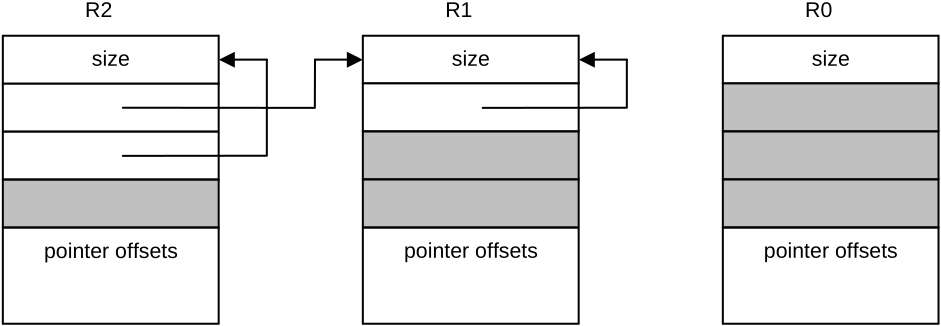
\includegraphics[width=.8\textwidth]{i/C/4.png}
  \caption{Type descriptors}
  \label{fig:typdesc}
\end{figure}

A type test of the form \verb|p IS T| then, consists of a comparison of the type tag of \verb|p^| at
address \verb|p-8| with the tag held in the descriptor of \verb|T| at the extension level of the type
of \verb|p^|. A type guard \verb|p(T)| is synonymous to the statement
\begin{verbatim}
  IF ~(p IS T) THEN abort END
\end{verbatim}

The following example features 3 record types with associated pointer types, and hence also 3 type
descriptors. Each descriptor is 5 words long. Their addresses, and therefore their tags, are 0, 20,
and 40 respectively.
\begin{verbatim}
   0 00000020 FFFFFFFF FFFFFFFF FFFFFFFF FFFFFFFF
  20 00000020 00014006 FFFFFFFF FFFFFFFF FFFFFFFF
  40 00000020 00014005 00028001 FFFFFFFF FFFFFFFF
  
  MODULE Pattern13;
    TYPE
      P0 = POINTER TO R0;
      P1 = POINTER TO R1;
      P2 = POINTER TO R2;
      R0 = RECORD x: INT END ;
      R1 = RECORD (R0) y: INT END ;
      R2 = RECORD (R1) z: INT END ;
    VAR
      p0: P0;                         60 
      p1: P1;                         64
      p2: P2;                         68
  BEGIN
    p0.x := 0;         LDR R0 SB 60                  
                       MOV R1 R0 0    p0.x          
                       STR R1 R0 0    no type check
    p1.y := 1;         LDR R0 SB 64   
                       MOV R1 R0 1    
                       STR R1 R0 4    p1.y
    p0(P1).y := 3;     LDR R0 SB 60   p0
                       LDR R1 R0 -8   tag(p0)
                       LDR R1 R1 4    
                       ADD R2 SB 20   TD P1
                       CMP R3 R2 R1
                       BLNE R12
                       MOV R1 R0 3
                       STR R1 R0 4    p0.z    
    p0(P2).z := 5;     LDR R0 SB 60   p0
                       LDR R1 R0 -8   tag(p0)
                       LDR R1 R1 8    
                       ADD R2 SB 40   TD P2
                       CMP R3 R2 R1   
                       BLNE R12       
                       MOV R1 R0 5    
                       STR R1 R0 8    p0.z
    IF p1 IS P2 THEN   LDR R0 SB 64   p1
                       LDR R1 R0 -8   tag(p1)
                       LDR R1 R1 8    
                       ADD R2 SB 40   TD P2
                       CMP R3 R2 R1
                       BNE 2
      p0 := p2         LDR R0 SB 68
                       STR R0 SB 60
    END
  END Pattern13.
\end{verbatim}

\subsection{RECORD extensions as VAR parameters}
Records occurring as VAR-parameters may also require a type test at program execution time. This is
because VAR-parameters effectively constitute hidden pointers. Type tests and type guards on
VAR-parameters are handled in the same way as for variables referenced via pointers, with a slight
difference, however. Statically declared record variables may be used as actual parameters, and they
are not prefixed by a type tag. Therefore, the tag has to be supplied together with the variable's
address when the procedure is called, i.e. when the actual parameter is established. Record structured
VAR-parameters therefore consist of address and type tag. This is similar to dynamic array descriptors
consisting of address and length.
\begin{verbatim}
   0 00000020 FFFFFFFF FFFFFFFF FFFFFFFF FFFFFFFF
  20 00000020 00014006 FFFFFFFF FFFFFFFF FFFFFFFF
  
  MODULE Pattern14;
    TYPE
      R0 = RECORD a, b, c: INT END ;
      R1 = RECORD (R0) d, e: INT END ;
    VAR
      r0: R0;                           40
      r1: R1;                           52
  
    PROC P(VAR r: R0);
    BEGIN             ...
      r.a := 1;       LDR R1 SP 4    r
                      STR R0 R1 0    r.a
      r(R1).d := 2    LDR R0 SP 8    tag(r)
                      LDR R0 R0 4    
                      ADD R1 SB 20   R1
                      CMP R2 R1 R0   
                      BLNE R12       
                      MOV R0 R0 2    
                      LDR R1 SP 4    r
                      STR R0 R1 12   r.d
    END P;            ...
  
  BEGIN               ...
    P(r0);            ADD R0 SB 40   r0
                      ADD R1 SB 0    tag(R0)
                      BL P           
    P(r1)             ADD R0 SB 52   r1
                      ADD R1 SB 20   tag(R1)
                      BL P
  END Pattern14.      ...
\end{verbatim}

\subsection{ARRAY assignments and strings}
\begin{verbatim}
  MODULE Pattern15;
    VAR s0, s1: ARRAY 32 OF CHAR;
  
    PROC P(x: ARRAY OF CHAR);
    END P;
  BEGIN
    s0 := "ABCDEF";   ADD R0 SB 0    @s0
                      ADD R1 SB 64   @"ABCDEF"
                      LDR R2 R1 0    
                      ADD R1 R1 4    
                      STR R2 R0 0    
                      ADD R0 R0 4    
                      ASR R2 R2 24   test for 0X
                      BNE -6         
    s0 := s1;         ADD R0 SB 0    @s0
                      ADD R1 SB 32   @s1
                      MOV R2 R0 8    len
                      LDR R3 R1 0    
                      ADD R1 R1 4    
                      STR R3 R0 0    
                      ADD R0 R0 4    
                      SUB R2 R2 1    
                      BNE -6         
    P(s1);            ADD R0 SB 32   @s1
                      MOV R1 R0 32   len
                      BL -38         P
    P("012345");      ADD R0 SB 72   @"012345"
                      MOV R1 R0 7    len (incl 0X)
                      BL -42         P
    P("%")            ADD R0 SB 80   @"%"
                      MOV R1 R0 2    len
                      BL -46         P
  END Pattern15.
\end{verbatim}

\subsection{Predeclared procedures}
\begin{verbatim}
  MODULE Pattern16;
    VAR m, n: INT; x: REAL; u: SET;
        a, b: ARRAY 10 OF INT;
        s, t: ARRAY 16 OF CHAR;
  BEGIN
    INC(m);              ADD R0 SB 0      @m             
                         LDR R1 R0 0      
                         ADD R1 R1 1      
                         STR R1 R0 0      
    DEC(n, 10);          ADD R0 SB 4      @n
                         LDR R1 R0 0      
                         SUB R1 R1 10     
                         STR R1 R0 0      
    INCL(u, 3);          ADD R0 SB 12     @u
                         LDR R1 R0 0      
                         OR R1 R1 8       {3}
                         STR R1 R0 0      
    EXCL(u, 7);          ADD R0 SB 12     @u
                         LDR R1 R0 0      
                         AND R1 R1 -129   -{7}
                         STR R1 R0 0      
    ASSERT(m < n);       LDR R0 SB 0      
                         LDR R1 SB 4      
                         CMP R0 R0 R1     
                         BLGE R12         
    UNPK(x, n);          LDR R0 SB 8      x
                         ASR R1 R0 23     
                         SUB R1 R1 127    
                         STR R1 SB 4      n
                         LSL R1 R1 23     
                         SUB R0 R0 R1     
                         STR R0 SB 8      x
    PACK(x, n);          LDR R0 SB 8      x
                         LDR R1 SB 4      n
                         LSL R1 R1 23     
                         ADD R0 R0 R1     
                         STR R0 SB 8      x
    s := "0123456789";   ADD R0 SB 96     @s
                         ADD R1 SB 128    adr of string
                         LDB R2 R1 0      loop
                         ADD R1 R1 4      
                         STB R2 R0 0      
                         ADD R0 R0 4      
                         ASR R2 R2 24     
                         BNE -6           
    IF s < t THEN        ADD R0 SB 96     @s
                         ADD R1 SB 112    @t
                         LDB R2 R0 0      loop
                         ADD R0 R0 1
                         LDB R3 R1 0
                         ADD R1 R1 1
                         CMP R4 R2 R3
                         BNE 2
                         CMP R4 R2 0
                         BNE -8
                         BGE 3
      m := 1             MOV R0 R0 1
                         STR R0 SB 0      m
    END
  END Pattern16.
\end{verbatim}

\subsection{Predeclared functions}
\begin{verbatim}
  MODULE Pattern17;
    VAR m, n: INT;
        x, y: REAL;
        b: BOOL; ch: CHAR;
  BEGIN
    n := ABS(m);      LDR R0 SB 0        m      
                      CMP R0 R0 0        
                      BGE 2              
                      MOV R1 R0 0        
                      SUB R0 R1 R0       
                      STR R0 SB 4        n
    y := ABS(x);      LDR R0 SB 8        x
                      LSL R0 R0 1        
                      ROR R0 R0 1        
                      STR R0 SB 12       y
    b := ODD(n);      LDR R0 SB 4        n
                      AND R0 R0 1        
                      BEQ 2              
                      MOV R0 R0 1        
                      B 1                
                      MOV R0 R0 0        
                      STB R0 SB 16       b
    n := ORD(ch);     LDB R0 SB 17       ch
                      STR R0 SB 4        n
    n := FLOOR(x);    LDR R0 SB 8        x
                      MOV' R1 R0 4B00H   
                      FAD" R0 R0 R1      floor
                      STR R0 SB 4        n
    y := FLT(m);      LDR R0 SB 0        m
                      MOV' R1 R0 4B00H   
                      FAD' R0 R0 R1      float
                      STR R0 SB 12       y
    n := LSL(m, 3);   LDR R0 SB 0        m
                      LSL R0 R0 3        
                      STR R0 SB 4        n
    n := ASR(m, 8);   LDR R0 SB 0
                      ASR R0 R0 8
                      STR R0 SB 4
    m := ROR(m, n);   LDR R0 SB 0
                      LDR R1 SB 4
                      ROR R0 R0 R1
                      STR R0 SB 0
  END Pattern17.
\end{verbatim}

\section{Internal data structures and module interfaces}
\subsection{Data structures}
In \S \ref{sec:cintro} it was explained that declarations inherently constitute context-dependence of
the translation process. Although parsing still proceeds on the basis of a context-free syntax and
relies on contextual information only in a few isolated instances, information provided by declarations
affects the generated code significantly. During the processing of declarations, their information is
transferred into the "\emph{symbol table}", a data structure of considerable complexity, from where
it is retrieved for the generation of code.

This dynamic data structure is defined in module ORB in terms of 2 record types called \verb|Object|
and \verb|Struct|. These types pervade all other modules with the exception of the scanner. They are
therefore explained before further details of the compiler are discussed (see module ORB below).

For each declared identifier an instance of type \verb|Object| is generated. The record holds the
identifier and the properties associated with the identifier given in its declaration. Since Oberon
is a statically typed language, every object has a type. It is represented in the record by its
\verb|typ| field, which is a pointer to a record of type \verb|Struct|. Since many objects may be of
the same type, it is appropriate to record the type's attributes only once and to refer to them via
a pointer. The properties of type \verb|Struct| will be discussed below.

The kind of object which a table entry represents is indicated by the field class. Its values are
denoted by declared integer constants: \verb|Var| indicates that the entry describes a variable,
\verb|Con| a constant, \verb|Fld| a record field, \verb|Par| a VAR-parameter, and \verb|Proc| a
procedure. Different kinds of entries carry different attributes. A variable or a parameter carries
an address, a constant has a value, a record field has an offset, and a procedure has an entry address,
a list of parameters, and a result type. For each class the introduction of an extended record type
would seem advisable. This was not done, however, for 3 reasons:
\begin{itemize}
  \item[$1^{st}$], the compiler was first formulated in (a subset of) Modula-2 which does not feature
      type extension.
  \item[$2^{nd}$], not making use of type extensions would make it simpler to translate the compiler
      into other languages for porting the language to other computers. And
  \item[$3^{rd}$], all extensions were known at the time the compiler was planned.
\end{itemize}
Hence extensibility provided no argument for the introduction of a considerable variety of types. The
simplest solution lies in using the multi-purpose fields \verb|val| and \verb|dsc| for class-specific
attributes. For example, \verb|val| holds
\begin{itemize}
  \item an address for variables, parameters, and procedures,
  \item an offset for record fields, and
  \item a value for constants.
\end{itemize}

The definition of a type yields a record of type \verb|Struct|, regardless of whether it occurs within
a type declaration, in which case also a record of type \verb|Object| (class=\verb|Typ|) is generated,
or in a variable declaration, in which case the type remains anonymous. All types are characterized by
a form and a size. A type is either a basic type or a constructed type. In the latter case it refers to
one or more other types. Constructed types are arrays, records, pointers, and procedural types. The
attribute form refers to this classification. Its value is an integer.

Just as different object classes are characterized by different attributes, different forms have
different attributes. Again, the introduction of extensions of type \verb|Struct| was avoided. Instead,
some of the fields of type \verb|Struct| remain unused in some cases, such as for basic types, and
others are used for form-specific attributes. For example, the attribute base refers to the element
type in the case of an array, to the result type in the case of a procedural type, to the type to which
a pointer is bound, or to the base type of a (extended) record type. The attribute \verb|dsc| refers
to the parameter list in the case of a procedural type, or to the list of fields in the case of
a record type.

As an example, consider the following declarations:
\begin{verbatim}
  CONST N = 100;
  TYPE  Ptr = POINTER TO Rec;
        Rec = RECORD n: INTEGER; p, q: Ptr END ;
  VAR   k: INTEGER;
        a: ARRAY N OF INTEGER;
  PROC P(x: INTEGER): INTEGER;
\end{verbatim}

The corresponding data structure is shown in Fig. \ref{fig:declrep}. For details, the reader is
referred to the program listing of module ORB and the respective explanations.
\begin{figure}[h!]
  \centering
  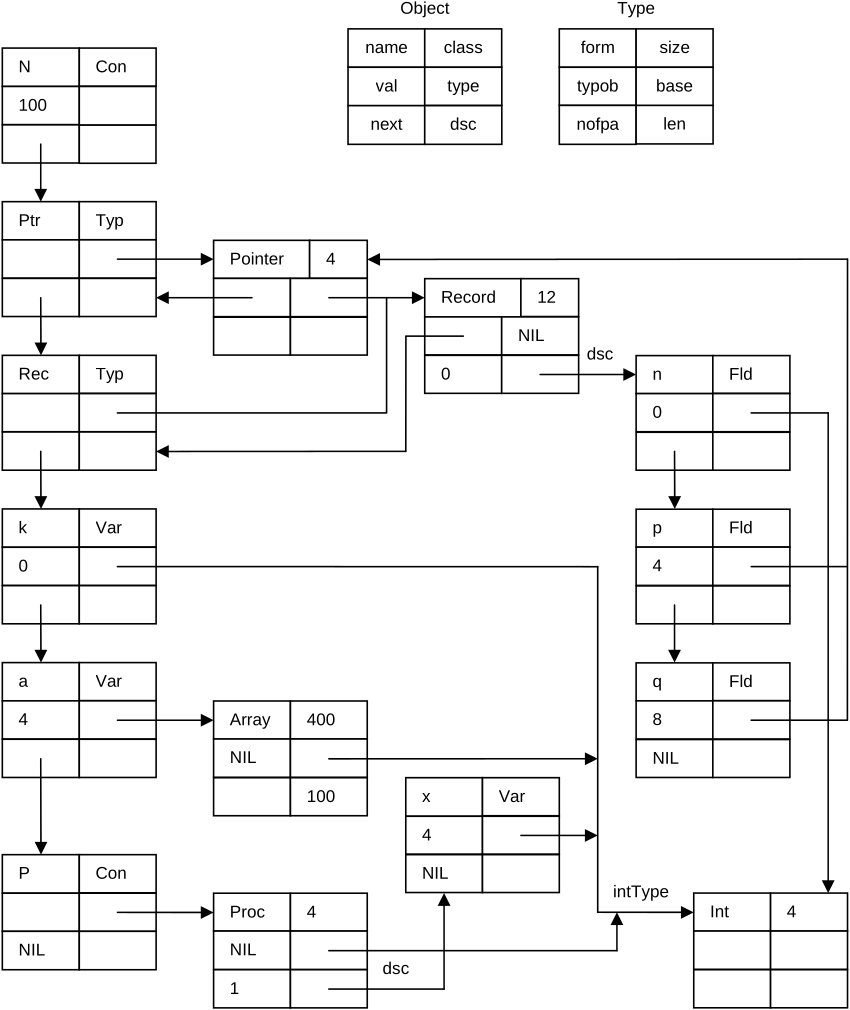
\includegraphics[width=.8\textwidth]{i/C/5.png}
  \caption{Representation of declarations}
  \label{fig:declrep}
\end{figure}

Only entries representing constructed types are generated during compilation. An entry for each basic
type is established by the compiler's initialization. It consists of an \verb|Object| holding the
standard type's identifier and a \verb|Struct| indicating its form, denoted by one of the values
\verb|Byte|, \verb|Bool|, \verb|Char|, \verb|Int|, \verb|Real|, or \verb|Set|. The object records
of the basic types are anchored in global pointer variables in module ORB (which actually should be
regarded as constants).

Not only are entries created upon initialization for basic types, but also for all standard procedures.
Therefore, every compilation starts out with a symbol table reflecting all standard, pervasive
identifiers and the objects they stand for.

We now return to the subject of \verb|Objects|. Whereas objects of basic classes (\verb|Const|,
\verb|Var|, \verb|Par|, \verb|Fld|, \verb|Typ|, \verb|SProc|, \verb|SFunc| and \verb|Mod|) directly
reflect declared identifiers and constitute the context in which statements and expressions are
compiled, compilations of expressions typically generate anonymous entities of additional, non-basic
modes. Such entities reflect selectors, factors, terms, etc., i.e. constituents of expressions and
statements. As such, they are of a transitory nature and hence are not represented by records allocated
on the heap. Instead, they are represented by record variables local to the processing procedures and
are therefore allocated on the stack. Their type is called \verb|Item| and is a slight variation of the
type \verb|Object|. Items are not referenced via pointers.

Let us assume, for instance, that a term \verb|x*y| is parsed. This implies that the operator and both
factors have been parsed already. The factors \verb|x| and \verb|y| are represented by 2 variables of
type \verb|Item| of \verb|Var| mode. The resulting term is again described by an item, and since the
product is transitory, i.e. has significance only within the expression of which the term is a
constituent, it is to be held in a temporary location, in a register. In order to express that an item
is located in a register, a new, non-basic mode \verb|Reg| is introduced.

Effectively, all non-basic modes reflect the target computer's architecture, in particular its
addressing modes. The more addressing modes a computer offers, the more item modes are needed to
represent them. The additional item modes required by the RISC processor are. They are declared in
module ORG:
\begin{table}[h!]
  \centering
  \begin{tabular}{l r}
    Reg  &   direct register mode \\
    RegI & indirect register mode \\
    Cond &    condition code mode
  \end{tabular}
\end{table}

The use of the types \verb|Object|, \verb|Item|, and \verb|Struct| for the various modes and forms,
and the meaning of their attributes are explained in the following tables:
\begin{table}[h!]
  \centering
  \begin{tabular}{r l c|c c c}
       & \multicolumn{2}{l}{Objects} & \multicolumn{3}{c}{Items} \\
       & class & val   & a     & b    & r \\\hline
     0 & Undef &      \\
     1 & Const & val   & val  \\
     2 & Var   & adr   & adr   & base \\
     3 & Par   & adr   & adr   & off  \\
     4 & Fld   & off   & off  \\
     5 & Typ   & TDadr & TDadr & modno\\
     6 & SProc & num  \\
     7 & SFunc & num  \\
     8 & Mod  \\      \\
    10 & Reg   &       &       &      & regno \\
    11 & RegI  &       & off   &      & regno \\
    12 & Cond  &       & Tjmp  & Fjmp & condition code
  \end{tabular}
\end{table}
\begin{table}[h!]
  \centering
  \begin{tabular}{r l c c c r}
       & \multicolumn{5}{l}{Structures} \\
       & form    & nofpar  & len      & dsc    & base \\\hline
     7 & Pointer &         &          &        &      base type \\
    10 & ProcTyp & nofpar  &          & param  &    result type \\
    12 & Array   &         & nofel    &        &   element type \\
    13 & Record  & ext lev & desc adr & fields & extension type
  \end{tabular}
\end{table}
Items have an attribute called \verb|lev| which is part of the address of the item. Positive values
denote the level of nesting of the procedure in which the item is declared; \verb|lev = 0| implies a
global object.  Negative values indicate that the object is imported from the module with number
\verb|-lev|.  The 3 types \verb|Object|, \verb|Item|, and \verb|Struct| are defined in module ORB,
which also contains procedures for accessing the symbol table.

\subsection{Module interfaces}
\label{ssc:modinf}
Before embarking on a presentation of the compiler's main module, the parser, an overview of its
remaining modules is given in the form of their interfaces. The reader is invited to refer to them
when studying the parser.

The interface of the scanner module ORS is simple. It defines the numeric values of all symbols.
But its chief constituent is procedure \verb|Get|. Each call yields the next symbol from the source
text, identified by an integer. Global variables represent attributes of the read symbol in certain
cases. If a number was read, \verb|ival| or \verb|rval| hold its numeric value. If an identifier or
a string was read, \verb|str| holds the ASCII values of the characters read.

Procedure \verb|Mark| serves to generate a diagnostic output indicating a brief diagnostic and the
scanner's current position in the source text. This procedure is located in the scanner, because only
the scanner has access to its current position. \verb|Mark| is called from all other modules.
\begin{verbatim}
  DEFINITION ORS; (*Scanner*)
    IMPORT Texts, Oberon;
  
    TYPE Ident = ARRAY 32 OF CHAR;
    VAR ival, slen: INT;
        rval: REAL;
        id: Ident;
        str: ARRAY 256 OF CHAR;
        errcnt: BOOL;
  
    PROC Mark (msg: ARRAY OF CHAR);
    PROC Get (VAR sym: INT);
    PROC Init (source: Texts.Text; pos: INT);
  END ORS.
\end{verbatim}

Module ORB defines the basic data structures representing declared objects and their types. It also
contains procedures for accessing these structures. \verb|NewObj| serves to insert a new identifier,
and it returns a pointer to the allocated object. \verb|ThisObj| returns the pointer to the object
whose name equals the global scanner variable \verb|ORS.id|. \verb|Thisimport| and \verb|thisfield|
deliver imported objects and record fields with names equal to \verb|ORS.id|.

Procedure \verb|Import| serves to read the specified symbol file and to enter its identifier in the
symbol table (class=\verb|Mod|). Finally, \verb|Export| generates the symbol file of the compiled
module, containing descriptions of all objects and structures marked for export.
\begin{verbatim}
  DEFINITION ORB; (*Base table handler*)
    TYPE
      Object = POINTER TO ObjDesc;
      Type = POINTER TO TypeDesc;
      ObjDesc = RECORD
        class, lev, exnp: INT;
        expo, rdo: BOOL;
        next, dsc: Object;
        type: Type;
        name: ORS.Ident;
        val: INT
      END ;
      TypeDesc = RECORD
        form, ref, mno: INT; (*ref for import/export only*)
        nofpar: INT; (*for records: extension level*)
        len: INT; (*for records: address of descriptor*)
        dsc, typobj: Object;
        base: Type;
        size: INT
      END ;
    VAR topScope: Object;
      byteType, boolType, charType, intType, realType,
      setType, nilType, noType, strType: Type;
  
    PROC Init;
    PROC Close;
    PROC NewObj (VAR obj: Object; id: ORS.Ident; class: INT);
    PROC thisObj (): Object;
    PROC thisimport (mod: Object): Object;
    PROC thisfield (rec: Type): Object;
    PROC OpenScope;
    PROC CloseScope;
    PROC Import (VAR modid, modid1: ORS.Ident);
    PROC Export (VAR modid: ORS.Ident;
                 VAR newSF: BOOL; VAR key: INT);
  END ORB.
\end{verbatim}

Module ORG contains the procedures for code generation. The names of these procedures indicate
the respective constructs for which code is to be produced. Note that an individual code generator
procedure is provided for every standard, predefined procedure. This is necessary, because they
generate in-line code.
\begin{verbatim}
DEFINITION ORG;
  CONST WordSize* = 4;
  TYPE Item* = RECORD
    mode*: INT;
    type*: ORB.Type;
    a*, b*, r: INT;
    rdo*: BOOL (*read only*)
  END ;
  VAR pc: INT;

  PROC MakeConstItem*(VAR x: Item; typ: ORB.Type; val: INT);
  PROC MakeRealItem*(VAR x: Item; val: REAL);
  PROC MakeStringItem*(VAR x: Item; len: INT);
  PROC MakeItem*(VAR x: Item; y: ORB.Object; curlev: INT);
  PROC Field*(VAR x: Item; y: ORB.Object); (* x := x.y *)
  PROC Index*(VAR x, y: Item); (* x := x[y] *)
  PROC DeRef*(VAR x: Item);
  PROC BuildTD*(T: ORB.Type; VAR dc: INT);
  PROC TypeTest*(VAR x: Item; T: ORB.Type; varpar, isguard: BOOL);

  PROC Not*(VAR x: Item); (* x := ~x, Boolean operators *)
  PROC And1*(VAR x: Item); (* x := x & *)
  PROC And2*(VAR x, y: Item);
  PROC Or1*(VAR x: Item); (* x := x OR *)
  PROC Or2*(VAR x, y: Item);

  PROC Neg*(VAR x: Item); (* x := -x, arithmetic operators *)
  PROC AddOp*(op: LONGINT; VAR x, y: Item); (* x := x +- y *)
  PROC MulOp*(VAR x, y: Item); (* x := x * y *)
  PROC DivOp*(op: INT; VAR x, y: Item); (* x := x op y *)
  PROC RealOp*(op: INT; VAR x, y: Item); (* x := x op y *)

  PROC Singleton*(VAR x: Item); (* x := {x}, set operators *)
  PROC Set*(VAR x, y: Item); (* x := {x .. y} *)
  PROC In*(VAR x, y: Item); (* x := x IN y *)
  PROC SetOp*(op: INT; VAR x, y: Item); (* x := x op y *)

  PROC IntRelation*(op: INT; VAR x, y: Item); (* x := x < y *)
  PROC SetRelation*(op: INT; VAR x, y: Item); (* x := x < y *)
  PROC RealRelation*(op: INT; VAR x, y: Item); (* x := x < y *)
  PROC StringRelation*(op: INT; VAR x, y: Item); (* x := x < y *)

  PROC StrToChar*(VAR x: Item); (*assinments*)
  PROC Store*(VAR x, y: Item); (* x := y *)
  PROC StoreStruct*(VAR x, y: Item); (* x := y *)
  PROC CopyString*(VAR x, y: Item); (*from x to y*)

  PROC VarParam*(VAR x: Item; ftype: ORB.Type); (*parameters*)
  PROC ValueParam*(VAR x: Item);
  PROC OpenArrayParam*(VAR x: Item);
  PROC StringParam*(VAR x: Item);

  PROC For0*(VAR x, y: Item); (*For Statements*)
  PROC For1*(VAR x, y, z, w: Item; VAR L: LONGINT);
  PROC For2*(VAR x, y, w: Item);

  (* Branches, procedure calls, procedure prolog and epilog *)
  PROC Here*(): LONGINT;
  PROC FJump*(VAR L: LONGINT);
  PROC CFJump*(VAR x: Item);
  PROC BJump*(L: LONGINT);
  PROC CBJump*(VAR x: Item; L: LONGINT);
  PROC Fixup*(VAR x: Item);
  PROC PrepCall*(VAR x: Item; VAR r: LONGINT);
  PROC Call*(VAR x: Item; r: LONGINT);
  PROC Enter*(parblksize, locblksize: LONGINT; int: BOOL);
  PROC Return*(form: INT; VAR x: Item; size: LONGINT; int: BOOL);

  (* In-line code procedures*)
  PROC Increment*(upordown: LONGINT; VAR x, y: Item);
  PROC Include*(inorex: LONGINT; VAR x, y: Item);
  PROC Assert*(VAR x: Item);
  PROC New*(VAR x: Item);
  PROC Pack*(VAR x, y: Item);
  PROC Unpk*(VAR x, y: Item);
  PROC Led*(VAR x: Item);
  PROC Get*(VAR x, y: Item);
  PROC Put*(VAR x, y: Item);
  PROC Copy*(VAR x, y, z: Item);
  PROC LDPSR*(VAR x: Item);
  PROC LDREG*(VAR x, y: Item);

  (*In-line code functions*)
  PROC Abs*(VAR x: Item);
  PROC Odd*(VAR x: Item);
  PROC Floor*(VAR x: Item);
  PROC Float*(VAR x: Item);
  PROC Ord*(VAR x: Item);
  PROC Len*(VAR x: Item);
  PROC Shift*(fct: LONGINT; VAR x, y: Item);
  PROC ADC*(VAR x, y: Item);
  PROC SBC*(VAR x, y: Item);
  PROC UML*(VAR x, y: Item);
  PROC Bit*(VAR x, y: Item);
  PROC Register*(VAR x: Item);
  PROC H*(VAR x: Item);
  PROC Adr*(VAR x: Item);
  PROC Condition*(VAR x: Item);

  PROC Open*(v: INT);
  PROC SetDataSize*(dc: LONGINT);
  PROC Header*;
  PROC Close*(VAR modid: ORS.Ident; key, nofent: LONGINT);
END ORG.
\end{verbatim}

\section{The Parser}
The main module ORP constitutes the parser. Its single command \verb|Compile| - at the end of the
program listing - identifies the source text according to the Oberon command conventions. It then
calls procedure \verb|Module| with the identified source text as parameter. The command forms are:
\begin{verbatim}
  ORP.Compile @	          The most recent selection identifies
                              the beginning of the source text.
  ORP.Compile ^	          The most recent selection identifies
                              the name of the source file.
  ORP.Compile f0 f1 ...   f0, f1, ... are the names of source files.
\end{verbatim}

File names and the characters \verb|@| and \verb|^| may be followed by an option specification
\verb|/s|. Option \verb|s| enables the compiler to overwrite an existing symbol file, thereby
invalidating clients.

The parser is designed according to the proven method of top-down, recursive descent parsing with
a look-ahead of a single symbol. The last symbol read is represented by the global variable sym.
Syntactic entities are mirrored by procedures of the same name. Their goal is to recognize the
specified construct in the source text. The start symbol and corresponding procedure is Module.
The principal parser procedures are shown in Fig. \ref{fig:pararch}, which also exhibits their calling
hierarchy.  Loops in the diagram indicate recursion in the syntactic definition.
\begin{figure}[h!]
  \centering
  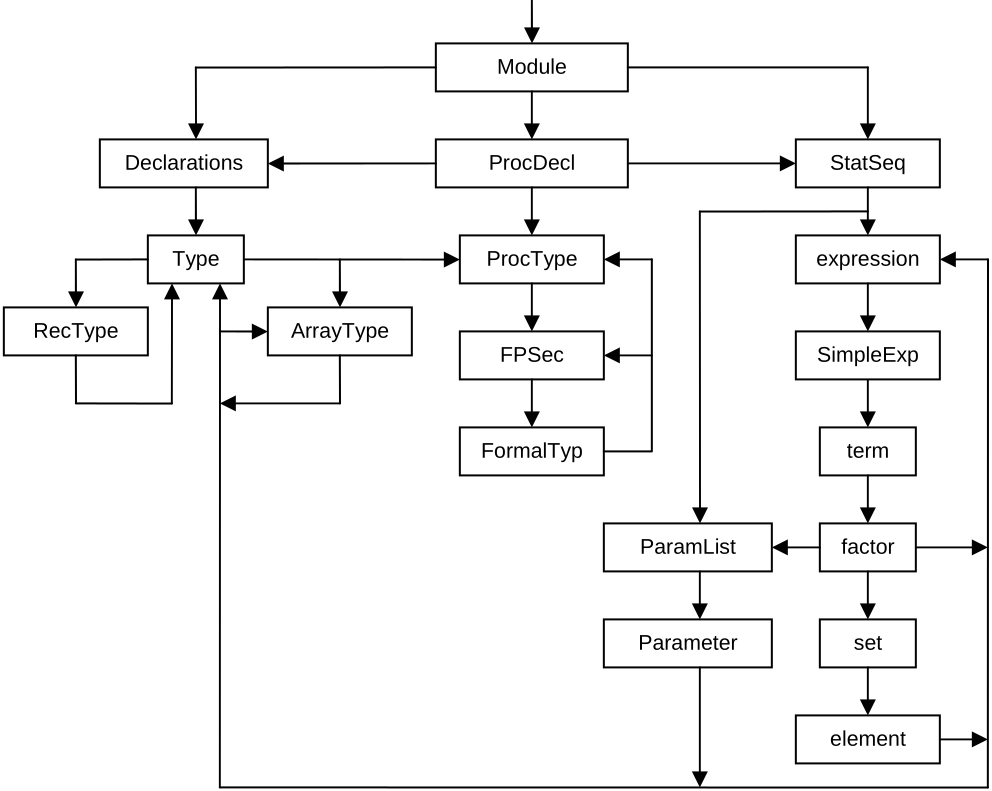
\includegraphics[width=\textwidth]{i/C/6.png}
  \caption{Parser procedure hierarchy}
  \label{fig:pararch}
\end{figure}

The rule of parsing strictly based on a single-symbol look-ahead and without reference to context is
violated in three places. The prominent violation occurs in statements. If the first symbol of a
statement is an identifier, the decision of whether an assignment or a procedure call is to be
recognized is based on contextual information, namely the class of the identified object. The
second violation occurs in qualident; if the identifier x preceding a period denotes a module, it is
recognized together with the subsequent identifier as a qualified identifier. Otherwise x supposedly
denotes a record variable. The third violation is made in procedure selector; if an identifier is
followed by a left parenthesis, the decision of whether a procedure call or a type guard is to be
recognized is again made on the basis of contextual information, namely the mode of the identified
object.

A fairly large part of the program is devoted to the discovery of errors. Not only should they be
properly diagnosed. A much more difficult requirement is that the parsing process should continue
on the basis of a good guess about the structure that the text should most likely have. The parsing
process must continue with some assumption and possibly after skipping a short piece of the
source text. Hence, this aspect of the parser is mostly based on heuristics. Incorrect assumptions
about the nature of a syntactic error lead to secondary error diagnostics. There is no way to avoid
them. A reasonably good result is obtained by the fact that procedure ORS.Mark inhibits an error
report, if it lies less than 10 characters ahead of the last one. Also, the language Oberon is
designed with the property that most large constructs begin with a unique symbol, such as IF,
WHILE, CASE, RECORD, etc. These symbols facilitate the recovery of the parsing process in the
erroneous text. More problematic are open constructs which neither begin nor end with key
symbols, such as types, factors, and expressions. Relying on heuristics, the source text is skipped
up to the first occurrence of a symbol which may begin a construct that follows the one being
parsed. The employed scheme may not be the best possible, but it yields quite acceptable results
and keeps the amount of program devoted to the handling of erroneous texts within justifiable
bounds.

Besides the parsing of text, the Parser also performs the checking for type consistency of objects.
This is based on type information held in the global table, gained during the processing of
declarations, which is also handled by the routines which parse. Thereby an unjustifiably large
number of very short procedures is avoided. However, the strict target-computer independence of
the parser is violated slightly: Information about variable allocation strategy including alignment, and
about the sizes of basic types is used in the parser module. Whereas the former violation is
harmless, because the allocation strategy is hardly controversial, the latter case constitutes a
genuine target-dependence embodied in a number of explicitly declared constants. Mostly these
constants are contained in the respective type definitions, represented by records of type Type
initialized by ORB. The following procedures allocate objects and generate elements of the symbol
table:
\begin{table}[h!]
  \centering
  \begin{tabular}{l l}
    Declarations         & Object(Con), Object(Typ), Object(Var) \\
    ProcedureDeclaration & Object(xProc) \\
    FormalType           & Object(Var), Object(Par) \\
    ORB.Import           & Object(Mod) \\
    RecordType           & Object(Fld), Type(Record) \\
    ArrayType            & Type(Array) \\
    ProcedureType        & Type(ProcTyp) \\
    Type                 & Type(Pointer) \\
    FormalType           & Type(Array)
  \end{tabular}
\end{table}

An inherently nasty subject is the treatment of forward references in a single-pass compiler. In
Oberon, there are 2 such cases:
\begin{enumerate}
  \item Forward declarations of procedures. They have been eliminated from the revision of the Oberon
    language in the year 2007 as they should be avoided if ever possible. If it is impossible, a remedy
    is to declare a variable of the given procedure type, and assign the procedure to be forwarded to
    this variable. The nastiness of procedure forward declarations originates in the necessity to
    specify parameters and result type in the forward declaration. These must be repeated in the actual
    procedure declaration, and one expects that a compiler verifies the equality (or equivalence) of
    the 2 declarations. This is a heavy burden for a case that very rarely occurs.
  \item Forward declarations of pointer types also constitutes a nasty exception, but its exclusion
    would be difficult to justify. If in a pointer declaration the base type (to which the pointer is
    bound) is not found in the symbol table, a forward reference is therefore automatically assumed.
    An entry for the pointer type is generated anyway (see procedure \verb|Type|) and an element is
    inserted in the list of pointer base types to be fixed up. This list is headed by the global
    variable \verb|pbsList|. When later in the text a declaration of a record type is encountered with
    the same identifier, the forward entry is recognized and the proper link is established (see
    procedure \verb|Declarations|).
\end{enumerate}

The compiler must check for undefined forward references when the current declaration scope is closed.
This check is performed at the end of procedure \verb|Declarations|.

The with statement had been eliminated from the language in its revision of 2007. Here it reappears
in the form of a case statement, whose cases are not labelled by integers, but rather by types. What
formerly was written as
\begin{verbatim}
  IF x IS T1 THEN
    WITH x: T1 DO ... x ... END
  ELSIF x IS T2 THEN
    WITH x: T2 DO ... x ... END
  ELSIF ...  END
\end{verbatim}
is now written more simply and more efficiently as
\begin{verbatim}
  CASE x OF
    T1: ... x ... |
    T2: ... x ... |
    ...  END
\end{verbatim}

where \verb|T1| and \verb|T2| are extensions of the type \verb|T0| of the case variable \verb|x|.
Compilation of this form of case statement merges the regional type guard of the former with statements
with the type test of the former if statements. This case statement represents the only case where a
symbol table entry - the type of \verb|x| - is modified during compilation of statements. When the end
of the with statement is reached, the change must be reverted.

\section{The scanner}
The scanner module ORS embodies the lexicographic definitions of the language, i.e. the definition
of abstract symbols in terms of characters. The scanner's substance is procedure Get, which scans
the source text and, for each call, identifies the next symbol and yields the corresponding integer
code. It is most important that this process be as efficient as possible. Procedure Get recognizes
letters indicating the presence of an identifier (or reserved word), and digits signalling the presence
of a number. Also, the scanner recognizes comments and skips them. The global variable ch
stands for the last character read.

A sequence of letters and digits may either denote an identifier or a key word. In order to determine
which is the case, a search is made in a table containing all key words for each would-be identifier.
This table is sorted alphabetically and according to the length of reserved words. It is initialized
when the compiler is loaded.

The presence of a digit signals a number. Procedure Number first scans the subsequent digits (and
letters) and stores them in a buffer. This is necessary, because hexadecimal numbers are denoted
by the postfix letter H (rather than a prefix character). The postfix letter X specifies that the
digits denote a character.

There exists one case in the language Oberon, where a look-ahead of a single character does not
suffice to identify the next symbol. When a sequence of digits is followed by a period, this period
may either be the decimal point of a real number, or it may be the first element of a range symbol (
.. ). Fortunately, the problem can be solved locally as follows: If, after reading digits and a period,
a second period is present, the number symbol is returned, and the look-ahead variable ch is
assigned the special value 7FX. A subsequent call of Get then delivers the range symbol.
Otherwise the period after the digit sequence belongs to the (real) number.

\section{Searching the symbol table, and handling symbol files}
\subsection{The structure of the symbol table}
The symbol table constitutes the context in which statements and expressions are parsed. Each
procedure establishes a scope of visibility of local identifiers. The records registering identifiers
belonging to a scope are linked as a linear list. They are of type \verb|Object|. Each object has a type.

Types are represented by records of type \verb|Type|. These 2 types pervade the entire compiler, and
they are defined as follows:
\begin{verbatim}
  TYPE Object = POINTER TO ObjDesc;
       Type   = POINTER TO TypeDesc;

  ObjDesc = RECORD
    class, lev, exno: INT;
    expo, rdo: BOOL; (*exported / read-only*)
    next, dsc: Object;
    type: Type;
    name: ORS.Ident;
    val: INT
  END ;

  TypeDesc = RECORD
    form, ref, mno: INT; (*ref is only used for import/export*)
    nofpar: INT; (*for procedures; extension level for records*)
    len: INT; (*for arrays, len < 0 => open array; for records: adr of descriptor*)
    dsc, typobj: Object;
    base: Type; (*for arrays, records, pointers*)
    size: INT; (*in bytes; always multiple of 4, except for Byte, Bool and Char*)
  END ;
\end{verbatim}

Procedures for generating and searching the lists are contained in module ORB. If a new identifier
is to be added, procedure NewObj first searches the list, and if the identifier is already present, a
double definition is diagnosed. Otherwise the new element is appended, thereby preserving the
order given by the source text.

Procedures, and therefore also scopes, may be nested. Each scope is represented by the list of its
declared identifiers, and the list of the currently visible scopes are again connected as a list.
Procedure OpenScope appends an element and procedure CloseScope removes it. The list of
scopes is anchored in the global variable topScope and linked by the field dsc. It is treated like a
stack. It consists of elements of type Object, each one being the header (class = Head) of the list of
declared entities. As an example, the procedure for searching an object (with name ORS.id) is
shown here:
\begin{verbatim}
  PROC thisObj*(): Object;
    VAR s, x: Object;
  BEGIN s := topScope;
    REPEAT x := s.next;
      WHILE (x # NIL) & (x.name # ORS.id) DO x := x.next END;
      s := s.dsc
    UNTIL (x # NIL) OR (s = NIL);
    RETURN x
  END thisObj;
\end{verbatim}

A snapshot of a symbol table for an example with nested scopes is shown in Fig. \ref{fig:symsnap}.
It is taken when the following declarations are parsed and when the statement \verb|S| is reached.
\begin{verbatim}
  VAR x: INT;
  
  PROC P(u: INT);
  BEGIN ... END P;
  
  PROC Q(v: INT);
    PROC R(w: INT);
    BEGIN S END R;
  BEGIN ... END Q;
\end{verbatim}

\begin{figure}[h!]
  \centering
  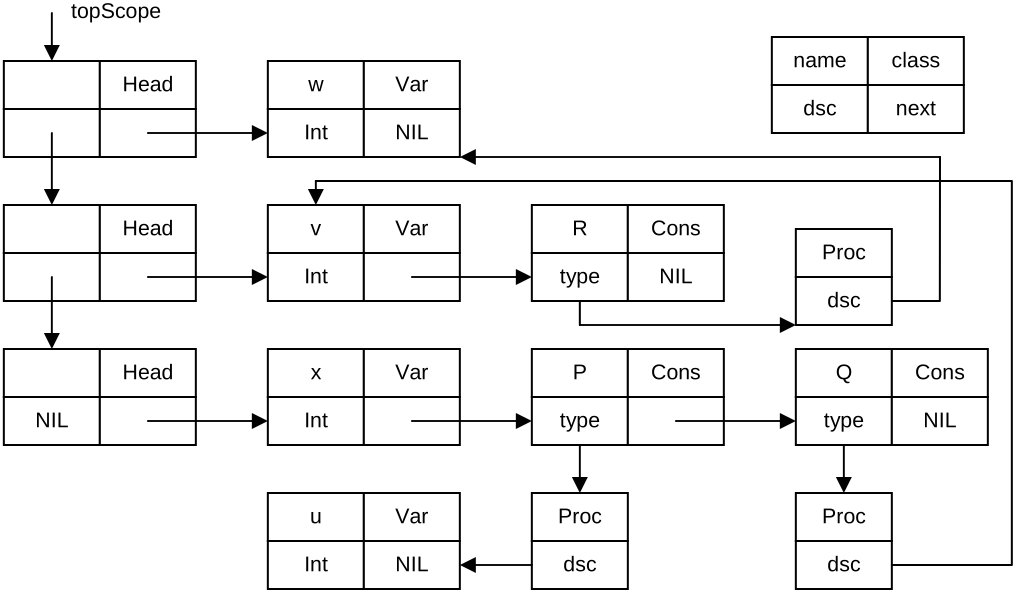
\includegraphics[width=\textwidth]{i/C/7.png}
  \caption{Snapshot of a symbol table}
  \label{fig:symsnap}
\end{figure}
A search of an identifier proceeds first through the scope list, and for each header its list of object
records is scanned. This mirrors the scope rule of the language and guarantees that if several
entities carry the same identifier, the most local one is selected. The linear list of objects represents
the simplest implementation by far. A tree structure would in many cases be more efficient for
searching, and would therefore seem more recommendable. Experiments have shown, however,
that the gain in speed is marginal. The reason is that the lists are typically quite short. The
superiority of a tree structure becomes manifest only when a large number of global objects is
declared. We emphasize that when a tree structure is used for each scope, the linear lists must still
be present, because the order of declarations is sometimes relevant in interpretation, e.g. in
parameter lists.

Not only procedures, but also record types establish their own local scope. The list of record fields
is anchored in the type record's field dsc, and it is searched by procedure thisField. If a record type
R1 is an extension of R0, then R1's field list contains only the fields of the extension proper. The
base type R0 is referenced by the BaseTyp field of R1. Hence, a search for a field may have to
proceed through the field lists of an entire sequence of record base types.

\subsection{Symbol files}
The major part of module ORB is devoted to input and output of symbol files. A symbol file is a
linearized form of an excerpt of the symbol table containing descriptions of all exported (marked)
objects. All exports are declared in the global scope. Procedure Export traverses the list of global
objects and outputs them to the symbol file.

The structure of a symbol file is defined by the syntax specified below. The following terminal
symbols are class and form specifiers or reference numbers for basic types with fixed values:

Classes: Con = 1, Var = 2, Par = 3, Fld = 4; Typ = 5

Forms: Byte = 1, Bool = 2, Char = 3, Int = 4, LInt = 5, Set = 6,
       Pointer = 7, NoTyp = 9, ProcTyp = 10, Array = 12, Record = 13

Syntax:
\begin{verbatim}
  SymFile = null key name versionkey {object}.
  object = (CON name type (value | exno) | TYP name type [{fix} 0] | VAR name type expno).
  type = ref (PTR type | ARR type len | REC type {field} 0 | PRO type {param} 0].
  field = FLD name type offset.
  param = (VAR | PAR) type.
\end{verbatim}

A procedure type description is contains a parameter list. Similarly, a record type description with
form specifier Record contains the list of field descriptions. Note that a procedure is considered as a
constant of a procedure type.

Objects have types, and types are referenced by pointers. These cannot be written on a file. The
straight-forward solution would be to use the type identifiers as they appear in the program to
denote types. However, this would be rather crude and inefficient, and second, there are
anonymous types, for which artificial identifiers would have to be generated.

An elegant solution lies in consecutively numbering types. Whenever a type is encountered the first
time, it is assigned a unique reference number. For this purpose, records (in the compiler) of type
Type contain the field ref. Following the number, a description of the type is then written to the
symbol file. When the type is encountered again during the traversal of the data structure, only the
reference number is issued, with negative sign. The global variable ORB.Ref functions as the
running reference number.

When reading a symbol file, a positive reference number is followed by the type's description. A
pointer to the type read is assigned to the global table typtab with the reference number as index.
When a negative reference number is read (it is not followed by a type description), then the type is
identified by \verb|typtab[-ref]| (see procedure \verb|InType|). In the following example, types are
identified by their reference number (e.g. \verb|R #14|), and later referenced by this number
(\verb|^14|).
\begin{verbatim}
MODULE A;
  CONST Ten* = 10; Dollar* = "\$";
  TYPE R* = RECORD u*: INT; v*: SET END ;
       S* = RECORD w*: ARRAY 4 OF R END ;
       P* = POINTER TO R;
       A* = ARRAY 8 OF INT;
       B* = ARRAY 4, 5 OF REAL;
       C* = ARRAY 10 OF S;
       D* = ARRAY OF CHAR;
  VAR x*: INT;
  PROC Q0*;
  BEGIN END Q0;
  PROC Q1*(x, y: INT): INT;
  BEGIN RETURN x+y END Q1;
END A.

class = CON Ten [^4] 10
class = CON Dollar [^3] 36
class = TYP R [#14 form = REC [^9] exno = 1 extlev = 0 size = 8 { v [^6] 4 u [^4] 0}]()
class = TYP S [#15 form = REC [^9] exno = 2 extlev = 0 size = 32 { w [#0 form = ARR [^14] len = 4 size = 32] 0}]()
class = TYP P [#16 form = PTR [^14]]()
class = TYP A [#17 form = ARR [^4] len = 8 size = 32]()
class = TYP B [#18 form = ARR [#0 form = ARR [^5] len = 5 size = 20] len = 4 size = 80]()
class = TYP C [#19 form = ARR [^15] len = 10 size = 320]()
class = TYP D [#20 form = ARR [^3] len = -1 size = 8]()
class = VAR x [^{}4] 3
class = CON Q0 [#0 form = PRO [^9]()] 4
class = CON Q1 [#0 form = PRO [^4]( class = VAR [^4] class = VAR [^4])] 5
\end{verbatim}

After a symbol file has been generated, it is compared with the file from a previous compilation of
the same module, if one exists. Only if the 2 files differ and if the compiler's s-option is enabled, is
the old file replaced by the new version. The comparison is made by comparing byte after byte
without consideration of the file's structure. This somewhat crude approach was chosen because of
its simplicity and yielded good results in practice.

A symbol file must not contain addresses (of variables or procedures). If they did, most changes in
the program would result in a change of the symbol file. This must be avoided, because changes in
the implementation (rather than the interface) of a module are supposed to remain invisible to the
clients. Only changes in the interface are allowed to effect changes in the symbol file, requiring
recompilation of all clients. Therefore, addresses are replaced by export numbers. The variable
exno (global in ORP) serves as running number (see ORP.Declarations and ORP.ProcedureDecl).
The translation from export number to address is performed by the loader. Every code file contains
a list (table) of addresses (of variables and entry points for procedures). The export number serves
as index in this table to obtain the requested address. Export numbers are generated by the parser.

Objects exported from some module M1 may refer in their declaration to some other module M0
imported by M1. It would be unacceptable, if an import of M1 would then also require the import of
M0, i.e. imply the automatic reading of M01's symbol file. It would trigger a chain reaction of imports
that must be avoided. Fortunately, such a chain reaction can be avoided by making symbol files
self-contained, i.e. by including in every symbol file the description of entities that stem from other
modules. Such entities are always types.

The inclusion of types imported from other modules seems simple enough to handle: type
descriptions must include a reference to the module from which the type was imported. This
reference is the name and key of the respective module. However, there exists one additional
complication that cannot be ignored. Consider a module M1 importing a variable x from a module
M0. Let the type T of x be defined in module M0. Also, assume M1 to contain a variable y of type
M0.T. Evidently, x and y are of the same type, and the compiler compiling M2 must recognize this
fact. Hence, when importing M0 during compilation of M1, the imported element T must not only be
registered in the symbol table, but it must also be recognized as being identical to the T already
imported from M2 directly. It is rather fortunate that the language definition specifies equivalence of
types on the basis of names rather than structure, because it allows type tests at execution time to
be implemented by a simple address comparison.

The measures to be taken to satisfy the new requirements are as follows:
\begin{enumerate}
  \item Every type element in a symbol file is given a module number. Before a type description is
    emitted to the file.
  \item If a type to be exported has a name and stems from another, imported module, then also the
    name and key of the module are attached, from which the type stems (see end of procedure
    \verb|ORB.OutType| and end of \verb|ORB.InType|).
\end{enumerate}

An additional detail is worth being mentioned here: Hidden pointers. We recall that individual fields
of exported record types may be hidden. If marked (by an asterisk) they are exported and therefore
visible in importing modules. If not marked, they are not exported and remain invisible, and
evidently seem to be omissible in symbol files. However, this is a fallacy. They need to be included
in symbol files, although without name, because of meta information to be provided for garbage
collection. This is elucidated as follows:

Assume that a module M1 declares a global pointer variables of a type imported from module M0.
\begin{verbatim}
  MODULE M0;
    TYPE Ptr = POINTER TO Rec0;
      Rec0* = RECORD p*, q: Ptr ... END ;
  END M0.
  
  MODULE M1;
    VAR p: M0.Ptr;
      r: RECORD f: M0.Ptr; ... END ;
  END M1.
\end{verbatim}

Here \verb|p| and \verb|r.f| are roots of data structures that must be visited by the garbage
collector. If they are not, they will not be marked, and therefore collected with disastrous and
entirely unpredictable consequences. The crux is that not only exported pointers (\verb|p.p|) must be
listed, but also hidden ones (\verb|p.q|), although they are not accessible in module \verb|M1|.

We chose to include hidden pointers in symbol files without their names, but with their type being of
the form ORB.NilTyp. This must be considered in procedure ORG.FindPtrs, where the condition
typ.form = ORB.Pointer must be extended to (typ.form = ORB.Pointer) OR (typ.form = ORB.NilTyp).

But the story does not end here. Assume that in the example above module M1 declares a type
Rec1 as a n extension of M0.Rec0. This requires the generation of a type descriptor. And this
descriptor must include not only field p, but also the hidden field q. This is achieved by also
extending the condition typ.form = ORB.Pointer in ORG.FindPtrFlds to (typ.form = ORB.Pointer)
OR (typ.form = ORB.NilTyp).

\section{The code generator}
The routines for generating instructions are contained in a single module: ORG. They are fairly
numerous, and therefore the interface of ORG is quite large. It is a procedural interface. This
implies that there is no "intermediate code" or "intermediate data structure" between parser and
code generator. This is one reason for the compactness of the code generator. The other is the
regularity and simplicity of the processor architecture. In order to understand the following material,
the reader is supposed to be familiar with this architecture (Appendix 2) and the generated code
patterns for individual language constructs (Section 12.2).

A distinguishing feature of this compiler is that parsing proceeds top-down according to the principle
of recursive descent in the parsing tree. This implies that for every syntactic construct a specific
procedure is called. It carries the same name as the construct. It also implies that properties of the
parsed construct can be represented by parameters of the parsing procedures. Consider, for
example, the construct of simple expression:
\begin{verbatim}
  SimpleExpression = term {"+" term}.
\end{verbatim}

The corresponding parsing procedure is
\begin{verbatim}
  PROC SimpleExpression(VAR x: Item);
    VAR y: Item;
  BEGIN term(x);
    WHILE sym = plus DO ORS.Get(sym); term(y); ORG.AddOp(x, y) END
  END SimpleExpression
\end{verbatim}

The generating procedure AddOp receives 2 parameters representing the operands, and returns
the result through the first parameter. This scheme carries the invaluable advantage of using
operands efficiently allocated on the stack rather than dynamically allocated on the heap and
subject to automatic storage retrieval (garbage collection). Here the processed operands quietly
disappear from the stack upon exit from the parser procedure.

The parameters representing syntactic constructs are of type Item defined in ORG. This data type
is rather similar to the type Object (in ORB). After all, it serves the same purpose; but it represents
internal items rather than declared objects.
\begin{verbatim}
  TYPE Item = RECORD
    mode: INT;
    type: ORB.Type;
    a, b, r: INT;
    rdo: BOOL (*read only*)
  END
\end{verbatim}

The attribute class of Object is renamed mode in Item. In fact, in some sense different classes
evoke different (corresponding) addressing modes as featured by the processor architecture.
According to the architecture, additional modes may have to be introduced. Thanks to the simplicity
of RISC, only three are needed:
\begin{verbatim}
Reg  = 10; The item x is located in register x.r
RegI = 11; The item x is addressed indirectly through register x.r plus offset x.a
Cond = 12; The item is represented by the condition bit registers
\end{verbatim}

Instructions are emitted sequentially and emitted by the four procedures Put0, Put1, Put2, Put3.
They directly correspond to the instruction formats of the RISC processor (see Chapter 11). The
instructions are stored in the array code and the compiler variable pc serves as running index.
\begin{verbatim}
  PROC Put0(op, a, b, c: INT);     format F0
  PROC Put1(op, a, b, im: INT);    format F1
  PROC Put2(op, a, b, off: INT);   format F2
  PROC Put3(op, cond, off: INT);   format F3
\end{verbatim}

\subsection{Expressions}
Expressions consist of operands and operators. They are evaluated and have a value. First, a
number of make-procedures transform objects into items (see Section 12.3.2). The principal one is
MakeItem. Typical objects are variables (class, mode = Var). Global variables are addressed with
base register SB (x.r = 13), local variables with the stack pointer SP (x.r = 14). VAR-parameters
are addressed indirectly; the address is on the stack (class, mode = Par, Ind). x.a is the offset from the stack pointer.

Before an operator can be applied to operands, these must first be transferred (loaded) into
registers. This is because the RISC performs operations only on registers. The loading is achieved
by procedure load (and loadAdr) in ORG. The resulting mode is Reg. In allocating registers, a strict
stack principle is used, starting with R0, up to R11. This is certainly not an optimal strategy and
provides ample room for improvement (usually called optimization). The compiler variable RH
indicates the next free register (top of register stack).

Base address SB is, as the name suggests, static. But this holds only within a module. It implies
that on every transfer to a procedure in another module, the static base must be adjusted. The
simplest way is to load SB before every external call, and to restore it to its old value after return
from the procedure. We chose a different strategy: loading on demand (see below: global
variables).

If a variable is indexed, has a field selector, is dereferenced, or has a type guard, this is detected
in the parser by procedure \verb|selector|. It calls generators \verb|Index|, \verb|Field|,
\verb|DeRef|, or \verb|TypeTest| accordingly (see \S \ref{ssc:modinf} and \S \ref{ssc:ptn1} - \S
\ref{ssc:ptn4}).  These procedures cause item modes to change as follows:
\begin{table}[h!]
  \centering
  \begin{tabular}{c c l l}
       & mode transition & instructions emitted & construct \\\hline
    1. & \multicolumn{3}{l}{Index(x, y) (y is loaded into y.r)} \\
       &  Var --> RegI   & \verb|ADD y.r, SP , y.r| & array variable \\
       &  Par --> RegI   & \verb|LDR RH , SP , x.a| & array parameter\\
       &                 & \verb|ADD y.r, RH , y.r|\\
       & RegI --> RegI   & \verb|ADD x.r, x.r, y.r| & indexed array \\\\

    2. & \multicolumn{3}{l}{Field(x, y) (y.mode = Fld, y.a = field offset)} \\
       &  Var --> Var    & none & field designator, add offset to \verb|x.a| \\
       & RegI --> RegI   & none & add field offset to \verb|x.a| \\
       &  Par --> Par    & none & add field offset to \verb|x.b| \\\\

    3. & \multicolumn{3}{l}{DeRef(x)} \\
       &  Var --> RegI   & \verb|LDR RH , SP , x.a| & dereferenced \verb|x^| \\
       &  Par --> RegI   & \verb|LDR RH , SP , x.a| & dereferenced parameter \verb|x^| \\
       &                 & \verb|LDR RH , RH , x.b| \\
       & RegI --> RegI   & \verb|LDR x.r, x.r, x.a|
  \end{tabular}
\end{table}

A fairly large number of procedures then deal with individual operators. Specifically, they are:
\begin{table}[h!]
  \centering
  \begin{tabular}{l l}
    operators & on \\\hline
    \verb|Not|, \verb|And1|, \verb|And2|, \verb|Or1|, \verb|Or2| & Booleans \\
    \verb|Neg|, \verb|AddOp|, \verb|MulOp|, \verb|DivOp|         & integers \\
    \verb|RealOp|                                                & real numbers \\
    \verb|Singleton|, \verb|Set|, \verb|In|, \verb|SetOp|        & Sets
  \end{tabular}
\end{table}

And finally, following the same pattern, are the procedures for relations (comparisons):
\begin{verbatim}
IntRelation, SetRelation, RealRelation, StringRelation.
\end{verbatim}
See Appendix for listing of ORG.

We note in particular that if all operands are constants, their evaluation is performed by the compiler
and not delegated to run-time.  This is an important efficiency factor.

\subsection{Relations}
RISC does not feature any compare instruction. Instead, subtraction is used, because an implicit
comparison wth 0 is performed along with any arithmetic (or load) instruction. Instead of \verb|x < y|
we use \verb|x-y < 0|. This is possible, because in addition to the computed difference deposited in a
register, also the result of the comparison is deposited in the condition flags \verb|N| (difference
negative) and \verb|Z| (difference zero). Relations therefore yield a result item \verb|x| with mode
\verb|Cond.x.r (= relmap[sym])| identifies the relation. Branch instructions (jumps) are executed
conditionally depending on these flags. The value \verb|x.r| is then used when generating branch
instructions. For example, the relation \verb|x < y| is translated simply into
\begin{verbatim}
  LDR R0, SP, x
  LDR R1, SP, y
  CMP R0, R0, R1
\end{verbatim}

and the resulting item mode is \verb|x.mode = Cond, x.r := "less"|. (The mnemonic CMP is synonymous
with SUB). More about relations and Boolean expressions will be explained in \S 12.7.6.

\subsection{Set operations}
The type SET represents sets of small integers in the range from 0 to 31. Bit \verb|i| being 1 signals
that \verb|i| is an element of the set. This is a convenient representation, because the logical
instructions directly mirror the set operations: \verb|AND| implements set intersection, \verb|OR| set
union, and \verb|XOR| the symmetric set difference. This representation also allows a simple and
efficient implementation of membership tests. The instructions for the expression \verb|n IN s| is
generated by procedure \verb|In|.  Assuming the value \verb|n| in register \verb|R0|, and the set
\verb|s| in \verb|R1|, we obtain
\begin{verbatim}
  ADD R0, R0, 1
  ROR R1, R1, R0   rotate s by i+1 position, the
                   relevant bit moving to the sign bit
\end{verbatim}

The resulting item mode is Cond with \verb|x.r = "minus"|.

Of some interest are the procedures for generating sets, i.e. for processing \verb|{m}|,
\verb|{m .. n}|, and \verb|{m, n}|, where \verb|m|, \verb|n| are integer expressions.

We start with \verb|{m}|. It is generated by procedure \verb|Singleton| using a shift instruction.
Assuming \verb|m| in \verb|R0|, the resulting code is
\begin{verbatim}
  MOV R1,  0, 1
  LSL R0, R1, R0   shift 1 by m bit positions to the left
\end{verbatim}

Somewhat more sophisticated is the generation of \verb|{m .. n}| by procedure \verb|Set|. Assuming
\verb|m| in \verb|R0|, and \verb|n| is \verb|R1|, the resulting code is
\begin{verbatim}
  MOV R2,  0, -2
  LSL R1, R2, R1   shift -2 by n bit positions to the left
  MOV R2,  0, -1
  LSL R0, R2, R0   shift -1 by m bit positions to the left
  XOR R0, R0, R1
\end{verbatim}

The set \verb|{m, n}| is generated as the union of \verb|{m}| and \verb|{n}|. If any of the element
values is a constant, several possibilities of code improvement are possible. For details, the reader
is referred to the source code of ORG.

\subsection{Assignments}
Statements have an effect, but no result like expressions. Statements are executed, not evaluated.
Assignments alter the value of variables through store instructions. The computation of the address
of the affected variable follows the same scheme as for loading. The value to be assigned must be
in a register.

Assignments of arrays (and records) are an exceptional case in so far as they are performed not by
a single store instruction, but by a repetition. Consider \verb|y := x|, where \verb|x|, and \verb|y|
are both arrays of \verb|n| integers. Assuming that the address of \verb|y| is in register \verb|R0|,
that of \verb|x| in \verb|R1|, and the value \verb|n| in \verb|R2|.  Then the resulting code is
\begin{verbatim}
L   LDR R3, R1, 0   source
    ADD R1, R1, 4
    STR R3, R0, 0   destination
    ADD R0, R0, 4
    SUB R2, R2, 1   counter
    BNE L
\end{verbatim}

\subsection{Conditional and repetitive statements}
These statements are implemented using branch instructions (jumps) as shown in \S \ref{ssc:ptn5} - \S
\ref{ssc:ptn7}. In all repetitive statements, backward jumps occur. Here, at the point of return the
value of the global variable \verb|ORG.pc| is saved in a local (!) variable of the involved parsing
procedure. It is retrieved when the backward jump is emitted. We note that branch instructions use
a displacement rather than an absolute destination address. It is the difference between the branch
instruction and the destination of the jump.

A difficulty, however, arises in the case of forward jumps, a difficulty inherent in all single-pass
compilers: When the branch is issued, its destination is still unknown. It follows that the branch
displacement must be later inserted when it becomes known, when the destination is reached. This
is called a \emph{fixup}. Here the method of fixup lists is used. The place of the instruction with
still unknown destination is held in a variable \verb|L| local to the respective parsing procedure.
If several branches have the same destination, \verb|L| is the heading of a list of the instructions
to be fixed up, with its links placed in the instructions themselves in the place of the eventual jump
displacement. This shown for the if statement by an excerpt of \verb|ORP.StatSequence| with local
variable \verb|L0|:
\begin{verbatim}
  ELSIF sym = ORS.if THEN
    ORS.Get(sym); ORG.FJump(L0); ORG.Fixup(x); expression(x);
    ORG.CFJump(x); Check(ORS.then, "no THEN"); StatSequence
    WHILE sym = ORS.elsif DO
      ORS.Get(sym); expression(x); ORG.CFJump(x);
      StatSequence; L0 := 0;
    END ;
    IF sym = ORS.else THEN ORS.Get(sym); ORG.FJump(L0); ORG.Fixup(x); StatSequence
    ELSE ORG.Fixup(x)
    END ;
    ORG.FixLink(L0);
\end{verbatim}

where in module ORG:
\begin{verbatim}
PROC CFJump(VAR x: Item); (*conditional forward jump*)
BEGIN
  IF x.mode # Cond THEN loadCond(x) END ;
  Put3(BC, negated(x.r), x.a); FixLink(x.b); x.a := pc-1
END CFJump;

PROC FJump(VAR L: LONGINT); (*unconditional forward jump*)
BEGIN Put3(BC, 7, L); L := pc-1
END FJump;

PROC fix(at, with: LONGINT);
BEGIN code[at] := code[at] DIV C24 * C24 + (with MOD C24)
END fix;

PROC FixLink(L: LONGINT);
  VAR L1: LONGINT;
BEGIN invalSB;
  WHILE L # 0 DO L1 := code[L] MOD 40000H; fix(L, pc-L-1); L := L1 END
END FixLink;

PROC Fixup(VAR x: Item);
BEGIN FixLink(x.a)
END Fixup;
\end{verbatim}

In while-, repeat-, and for- statements essentially the same technique is used with the support of the
identical procedures in ORG.

\subsection{Boolean expressions}
In the case of arithmetic expressions, our compilation scheme results in a conversion from infix to
postfix notation (\verb|x+y| => \verb|xy+|). This is not applicable for Boolean expressions, because
the operators \verb|&| and \verb|OR| are defined as follows:
\begin{verbatim}
  x  & y --> if x then y else FALSE
  x OR y -- > if x then TRUE else y
\end{verbatim}

This entails that depending on the value of \verb|x|, \verb|y| must not be evaluated. As a consequence,
jumps may have to be taken across the code for \verb|y|. Therefore, the same technique of conditional
evaluation must be used as for conditional statements. In the case of an expression \verb|x & y|
(\verb|x OR y|), procedure \verb|ORG.And1| resp. \verb|ORG.Or1| must be called just after parsing
\verb|x| (see \verb|ORP.term| resp. \verb|ORP.SimpleExpression|). Only after parsing also \verb|y| can
the generators \verb|ORG.And2| resp. \verb|ORG(Or2)| be called, providing the necessary fixups of
forward jumps.
\begin{verbatim}
PROC And1(VAR x: Item); (* x := x & *)
BEGIN
  IF x.mode # Cond THEN loadCond(x) END ;
  Put3(BC, negated(x.r), x.a); x.a := pc-1; FixLink(x.b); x.b := 0
END And1;

PROC And2(VAR x, y: Item);
BEGIN
  IF y.mode # Cond THEN loadCond(y) END ;
  x.a := merged(y.a, x.a); x.b := y.b; x.r := y.r
END And2;
\end{verbatim}

A negative consequence of this scheme having condition flags in the processor is that when an item
with mode \verb|Cond| has to be transferred into mode \verb|Reg|, as in a Boolean assignment, an
unpleasantly complex instruction sequence must be generated.  Fortunately, this case occurs quite
rarely.

\subsection{Procedures}
Before embarking on an explanation of procedure calls, entries and exits, we need to know how
recursion is handled and how storage for local variables is allocated. Procedure calls cause a
sequence of frames to be allocated in a stack fashion. These frames are the storage space for local
variables. Each frame is headed by a single word containing the return address of the call. This
address is deposited in R15 by the call instructions (BL, branch and link). The compiler "knows" the
size of the frame to be allocated, and thus merely decrements the stack pointer SP (R14) by this
amount. Upon return, SP is incremented by the same amount, and PC is restored by a branch
instruction. In the following example, a procedure P is called, calling itself Q, and Q calling P again
(recursion). The stack then contains 3 frames (see Fig. \ref{fig:stackfrm}).
\begin{figure}[h!]
  \centering
  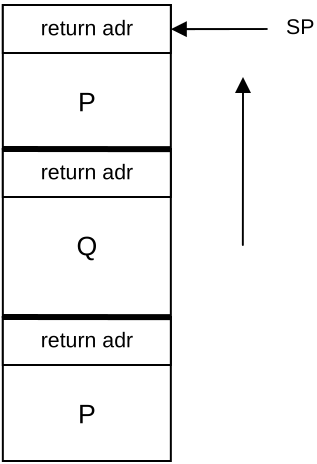
\includegraphics[width=.4\textwidth]{i/C/8.png}
  \caption{Stack frames}
  \label{fig:stackfrm}
\end{figure}

Scheme and layout determine the code sequences for call, entry and exit of procedures. Here is an
example of a procedure \verb|P| with 2 parameters:
\begin{verbatim}
Call:   LDR R0, param0   
        LDR R1, param1
        BL  P
        
Prolog: SUB SP , SP, size   decrement SP        
        STR LNK, SP, 0      push return adr
        STR R0 , SP, 4      push parameter 0
        STR R1 , SP, 8      push parameter1 ...
                           
Epilog: LDR LNK, SP, 0      pop return adr
        ADD SP , SP, size   increment SP
        BR  LNK
\end{verbatim}

When the call instruction is executed, parameters reside in registers, starting with R0. For function
procedures, the result is passed in register R0. This scheme is very efficient; storing the parameters
occurs only in a single place, namely at procedure entry, and not before each call. However, it has
severe consequences for the entire register allocation strategy. Throughout the compiler, registers
must be allocated in strict stack fashion. Furthermore, parameter allocation must start with R0. This
is a distinct drawback for function calls. If registers are occupied by other values loaded prior to
the call, they must be cleared, i.e. the parameters must be saved and reloaded after return. This is
rather cumbersome (see procedures \verb|ORG.SaveRegisters| and \verb|ORG.RestoreRegisters|).
\begin{verbatim}
F(x)           no register saving        
x + F(x)        
F(F(x))         
(x+1) + F(x)   register saving necessary
\end{verbatim}

\subsection{Type extension}
Static typing is an important principle in programming languages. It implies that every constant,
variable or function is of a certain data type, and that this type can be derived by reading the
program text without executing it. It is the key principle to introduce important redundancy in
languages in such a form that a compiler can detect inconsistencies. It is therefore the key element
for reducing the number of errors in programs.

However, it also acts as a restriction. It is, for example, impossible to construct data structures
(arrays, trees) with different types of elements. In order to relax the rule of strictly static typing,
the notion of \emph{type extension} was introduced in Oberon.  It makes it possible to construct
inhomogeneous data structures without abandoning type safety. The price is that the checking of type
consistency must in certain instances be deferred to runtime. Such checks are called \emph{type tests}.
The challenge is to defer to run-time as few checks as possible and as many as needed.

The solution in Oberon is to introduce families of types, and compatibility among their members.
Their members are thus related, and a family forms a hierarchy. The principle idea is the following:
Any record type T0 can be extended into a new type T1 by additional record fields (attributes). T1 is
then called an extension of T0, which in turn is said to be T1’s \emph{base type}. T1 is then type
compatible with T0, but not vice-versa. This property ensures that in many cases static type
checking is still possible. Furthermore, it turns out that run-time tests can be made very efficient,
thus minimizing the overhead for maintaining type safety.

For example, given the declarations
\begin{verbatim}
  TYPE R0 = RECORD u, v: INT END ;
       R1 = RECORD (R0) w: INT END
\end{verbatim}

we say that \verb|R1| is an \emph{extension} of \verb|R0|. \verb|R0| has the fields \verb|u| and
\verb|v|, \verb|R1| has \verb|u|, \verb|v|, and \verb|w|. The concept becomes useful in combination
with pointers. Let
\begin{verbatim}
  TYPE P0 = POINTER TO R0;
       P1 = POINTER TO R1;
  VAR p0: P0; p1: P1;
\end{verbatim}

Now it is possible to assign \verb|p1| to \verb|p0| (because a \verb|P1| is always also a \verb|P0|),
but not \verb|p0| to \verb|p1|, because a \verb|P0| need not be a \verb|P1|. This has the simple
consequence that a variable of type \verb|P0| may well point to an extension of \verb|R0|. Therefore,
data structures can be declared with a base type, say \verb|P0|, as common element type, but in fact
they can individually differ, they can be any extension of the base type.

Obviously, it must be possible to determine the actual, current type of an element even if the base
type is statically fixed. This is possible through a \emph{type test}, syntactically a Boolean factor:
\begin{verbatim}
  p0 IS P1   (short for p0^ IS R1)
\end{verbatim}

Furthermore, we introduce the \emph{type guard}. In the present example, the designator \verb|p0.w|
is illegal, because there is no field \verb|w| in a record of type \verb|R0|, even if the current value
of \verb|p0^| is a \verb|R1|. As this case occurs frequently, we introduce the short notation
\verb|p0(P1).w|, implying a test \verb|p0 IS P1| and an abort if the test is not met.

It is important to mention that this technique also applies to formal variable parameters of record
type, as they also represent a pointer to the actual parameter. Its type may be any extension of the
type specified for the formal parameter in the procedure heading.

How are type test and type guard efficiently implemented? Our first observation is that they must
consist of a single comparison only, similar to index checks. This in turn implies that types must be
identified by a single word. The solution lies in using the unique address of the type descriptor of
the (record) type. Which data must this descriptor hold? Essentially, type descriptors (TD) must
identify the base types of a given type. Consider the following hierarchy:
\begin{verbatim}
  TYPE T   = RECORD      … END ;
       T0  = RECORD (T ) … END ;   extension level 1 
       T1  = RECORD (T ) … END ;
       T00 = RECORD (T0) … END ;   extension level 2
       T01 = RECORD (T0) … END ;
       T10 = RECORD (T1) … END ;
       T11 = RECORD (T1) … END ;
\end{verbatim}
\begin{figure}[h!]
  \centering
  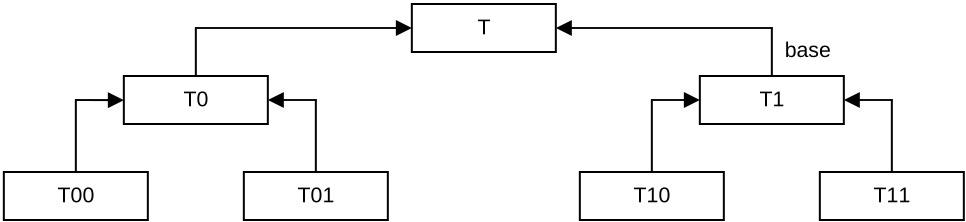
\includegraphics[width=.9\textwidth]{i/C/9.png}
  \caption{A type hierarchy}
  \label{fig:typarch}
\end{figure}

In the symbol table, the field \emph{base} refers to the ancestor of a given record type. Thus base of
the type representing \verb|T11| points to \verb|T1|, etc. Run-time checks, however, must be fast, and
hence cannot proceed through chains of pointers. Instead, each TD contains an array with references to
the ancestor TDs (including itself). For the example above, the TDs are as follows:
\begin{verbatim}
  TD(T  ) = [T         ]     
  TD(T0 ) = [T, T0     ]
  TD(T1 ) = [T, T1     ]
  TD(T00) = [T, T0, T00]
  TD(T01) = [T, T0, T01]
  TD(T10) = [T, T1, T10]
  TD(T11) = [T, T1, T11]
\end{verbatim}

Evidently, the first element can be omitted, as it always refers to the common base of the type
hierarchy. The last element always points to the TD’s owner. TDs are allocated in the data area, the
area for variables.

References to TDs are called \emph{type tags}. They are required in 2 cases.
\begin{itemize}
  \item[$1^{st}$] is for records referenced by pointers. Such dynamically allocated records carry an
    additional, hidden field holding their type tag. (A second additional word is reserved for use by
    the garbage collector. The offset of the tag field is therefore -8).
  \item[$2^{nd}$] case is that of record-typed VAR-parameters. In this case the type tag is explicitly
    passed along with the address of the actual parameter. Such parameters therefore require 2
    words/registers.
\end{itemize}

A type test then consists of a test for equality of 2 type tags. In \verb|p IS T| the first tag is that
of the n’th entry of the TD of \verb|p^|, where n is the extension level of \verb|T|. The second tag is
that of type \verb|T|. This is shown in \S \ref{ssc:ptn12} (see also Fig. \ref{fig:typdesc}).
The test then is as follows:
\begin{verbatim}
  p^.tag^[n] = adr(T)   n is the extension level to T
\end{verbatim}

When declaring a record type, it is not known how many extensions, nor how many levels will be
built on this type. Therefore TD’s should actually be infinite arrays. We decided to restrict them to 3
levels only. The first entry, which is never used for checking, is replaced by the size of the record.

\subsection{Import and export, global variables}
Addresses of imported objects are not available to the compiler. Their computation must be left to
the module loader (see Chapter 6). Similar to handling addresses of forward jumps, the compiler
puts the necessary information in place of the actual address into the instruction itself. In the case
of procedure calls, this is quite feasible, because the BL instruction features an offset field of 24
bits. The information consists of the module number and the export number of the imported object.
In addition, there is a link to the previous instruction referring to an imported procedure. The origin
of the list of procedure call fixups is rooted in the compiler variable fixorgP, and of the 24 bits in
each BL instruction 4 bits are used for the module number, 8 bits for the object's export number,
and 12 for the link. The loader need only scan this list to fix up the addresses (jump offsets).

Matters are more complex in the case of data. Object records in the symbol table have a field lev. It
indicates the nesting level of variables local to procedures. It is also used for the module number in
the case of variables of imported modules. Note that when importing, objects designating modules
are inserted in the symbol table, and the list of their own objects are attached in the field dsc. In
this latter case, the module numbers have an inverted sign (are negative). Such imported objects are
static, i.e. have a fixed address. In principle their absolute address could be computed (fixed) by the
module loader. However, this is not practicable, because RISC instructions have an address offset
of 16 bits only. It is therefore necessary in the general case to use a base address in conjunction
with the offset. We use a single register for holding the static base (SB, R13). This register need be
reloaded for every access to an imported variable. However, the compiler keeps track of external
accesses; if a variable is to be accessed from the same module as the previous case, then
reloading is avoided (see procedure \verb|GetSB| and global compiler variable \verb|curSB|).

This base address is fetched from a table global to the entire system. This module table contains
one entry for every module loaded, namely the address of the module's data section. The address
of the table is permanently in register MT(=R12). An access to an imported variable therefore
always requires 2 instructions:
\begin{verbatim}
  LDR SB, MT, modno*4   base address of data section
  LDR R0, SB, offset    offset computed by the loader from object's export number
\end{verbatim}

Considering the fact that references to external variables are (or should be) rare, this circumstance
is of no great concern. (Note also that such accesses are read-only). More severe is the fact that
we also treat global variables contained in the same module by the same technique. Their level
number is 0. One might use a specific base register for the base of the current module. Its content
would then have to be reloaded upon every procedure call and after every return. This is common
technique, but we have here chosen to reload only when necessary, i.e. only when an access is at
hand. This strategy rewards the programmer who sensibly uses global variables rarely.

\subsection{Traps}
This compiler provides an extensive system of safeguard by providing run-time checks (aborts) in
several cases:
\begin{table}[h!]
  \centering
  \begin{tabular}{c l}
    trap number & trap cause \\\hline
    1 & array index out of range \\
    2 & type guard failure \\
    3 & array or string copy overflow \\
    4 & access via NIL pointer \\
    5 & illegal procedure call \\
    6 & integer division by zero \\
    7 & assertion violated
  \end{tabular}
\end{table}

These checks are implemented very efficiently in order not to downgrade a program's performance.
Involved is typically a single compare instruction, plus a conditional branch (BLR MT). It is assumed
that entry 0 of the module table contain not a base address (module numbers start with 1), but a
branch instruction to an appropriate trap routine. The trap number is encoded in bits 4:7 of the
branch instruction.

The predefined procedure \verb|Assert| generates a conditional trap with trap number 7. For example,
the statement \verb|Assert(m = n)| generates
\begin{verbatim}
  LDR R0, m
  LDR R1, n
  CMP R0, R0, R1
  BLR 1 , 7CH   branch and link if unequal through R12, trap #7
\end{verbatim}

Procedure \verb|New|, representing the operator \verb|NEW|, has been implemented with the aid of the
trap mechanism. (This is in order to omit in ORG any reference to module Kernel, which contains the
allocation procedure \verb|New|). The generated code for the statement \verb|NEW(p)| is
\begin{verbatim}
  ADD R0, SP, p     address of p                                                    
  ADD R1, SB, tag   type tag
  BLR 7 , 0CH       branch and link unconditionally through R12(MT), trap #0
\end{verbatim}
